%class
	\documentclass{beamer}

%template
	\usetheme{HannoverSalman}
	\setbeamertemplate{navigation symbols}{}
	%\setbeamertemplate{footline}{\centering{\insertframenumber/\insertpresentationendpage}}
	%\setbeamertemplate{footline}{\hspace*{.5cm}\scriptsize{\hfill\insertframenumber\hspace*{.5cm}}} 


%packages
	\usepackage{amsmath, amssymb, graphicx,cancel}
	\usepackage[absolute,overlay]{textpos}
	\usepackage{subfigure}
	\usepackage{caption}\captionsetup{labelformat=empty,labelsep=none}
	\usepackage{geometry}
	\geometry{verbose}
	\usepackage{color}
	\usepackage{xmpmulti}
	\usepackage[3D]{movie15}
	\usepackage{hyperref}
%	\usepackage{bookmark}
	\usepackage[open,openlevel=4,atend]{bookmark}
	%\bookmarksetup{color=blue}
	\usepackage{multirow}
	\usepackage[style=numeric,defernumbers, authoryear]{biblatex}
	%\usepackage[square,sort]{natbib}
	%\usepackage{fancyhdr}%\pagestyle{fancy} 

	
	\hypersetup{bookmarksdepth = 4}


%citations files
	\bibliography{MyCitations}

%logoCSIPCPL
    \setlength{\TPHorizModule}{1mm}
    \setlength{\TPVertModule}{1mm}
    \newcommand{\logoCSIPCPL}
    {
    	\begin{textblock}{1}(100,2) %(100,85)  for bottom
    		
\includegraphics[width=1.5cm]{figs/logo_CSIP}
    	\end{textblock}
    	
	\begin{textblock}{1}(117,1) %(117,85)  for bottom
    		
\includegraphics[width=1.0cm]{figs/logo_CPL}
    	\end{textblock} 
    }

%logo evolution
    \newcommand{\logoEvolution}
    {    	
	\begin{textblock}{1}(110,1) %(117,85)  for bottom
    		\includegraphics[width=0.65in]{figs/logo_evolution.pdf}
    	\end{textblock} 
    }

%logo Qualcomm
    \newcommand{\logoQualcomm}
    {
    	\begin{textblock}{1}(110,2) %(100,85)  for bottom
    		\includegraphics[width=1.5cm]{figs/logo_qualcomm.jpg}
    	\end{textblock}
    }
%logo Qualcomm (long)
    \newcommand{\logoQualcommllong}
    {
    	\begin{textblock}{1}(0,0) 
    		\includegraphics[width=1.25in]{figs/logo_qualcomm_long.jpg}
    	\end{textblock}
    }

%logo Tech Tower
    \newcommand{\logoTechTower}
    {
    	\begin{textblock}{1}(0,0) 
    		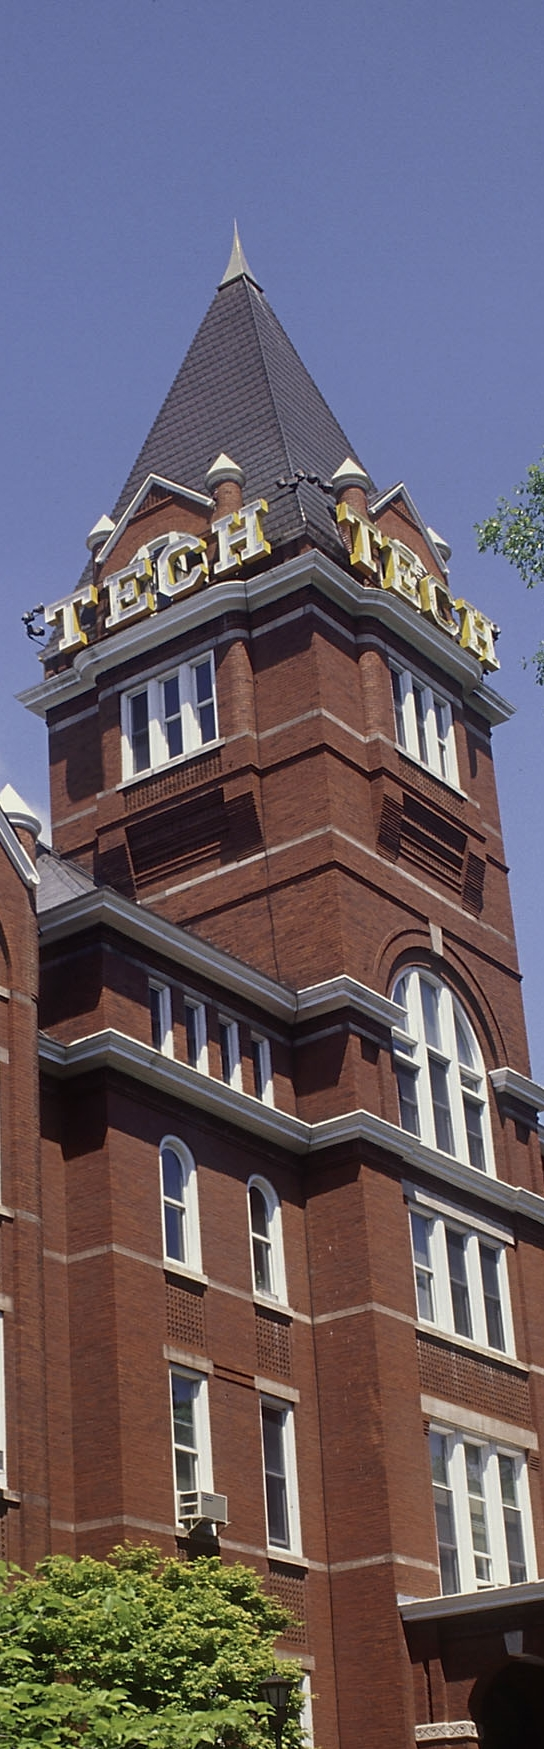
\includegraphics[width=1.25in]{figs/logo_TechTower.jpg}
    	\end{textblock}
    }

%logo tree
    \newcommand{\logoTree}
    {
    	\begin{textblock}{1}(0,0) 
    		\includegraphics[width=1.25in]{figs/logo_tree.jpg}
    	\end{textblock}
    }
%page numbers
    \newcommand{\mypagenum}
    {
    	\begin{textblock}{1}(1,94) 
		{\tiny \color[rgb]{0.2,0.2,1}\insertframenumber} %\insertframenumber,\insertpresentationendpage, \inserttotalframenumber
    	\end{textblock}
    }
%my footnote citation
	\newcommand{\myFootnoteCitation}[2]
	{
		\footnote{\tiny \citeauthor{#1}, \emph{#2}, \citeyear{#1}.}  %\citeauthor{#1}, \citetitle{#1}, #2 \citeyear{#1}.
	}
%my refer to citation
	\newcommand{\mycite}[1]
	{
		\emph{\citeauthor{#1} (\citeyear{#1})}
	}
%my footnote website citation
	\newcommand{\myFootnoteWebsiteCitation}[1]
	{
		\footnote{\tiny \citeauthor{#1}}
	}

\let\thefootnote\relax\footnotetext{Footnotetext without footnote mark}


%section underline
%\newcommand{\tmpsection}[1]{}
%\let\tmpsection=\section
%\renewcommand{\section}[1]{\tmpsection{\underline{#1}}}



%commands
	\newcommand{\likelihood}{p(Z_k| x_k) }						%likelihood
	\newcommand{\prior}{p(x_k)  } 								%prior
	\newcommand{\posterior} {p(x_k| Z_k)}						%posterior
	\newcommand{\prediction} {p(x_k| Z_{k-1})}					%prediction
	\newcommand{\update} {p(x_k|Z_k)}							%update
	\newcommand{\observations} {p(Z_k)}						%observations
	\newcommand{\prevobservations} {p(Z_{k-1})}				%previous observations
	\newcommand{\dxpk} {dx_{k-1}}							%dx_{k-1}
	\newcommand{\ChapKolm}{\int{p(x_k| x_{k-1})p(x_{k-1}|Z_{k-1})} \dxpk} %Chapman Kolmogorov

	%algorithm specific: JPDAF
	\newcommand{\likelihoodJPDAF}{p(Z_k| \chi, m, Z_{k-1}) }		%1. likelihood
	\newcommand{\priorJPDAF}{p(\chi|m, Z^{k-1}} 				%2. prior	
	\newcommand{\observationsJPDAF} {p(Z_k}					%3. observations
	\newcommand{\posteriorJPDAF} {p(\chi| Z_k)}					%4. posterior

%environments
	\newenvironment{changemargin}[2]
	{
	  	\begin{list}{}
		{
			\setlength{\topsep}{0pt}%
			\setlength{\leftmargin}{#1}%
			\setlength{\rightmargin}{#2}%
			\setlength{\listparindent}{\parindent}%
			\setlength{\itemindent}{\parindent}%
			\setlength{\parsep}{\parskip}%
		}
	  	\item[]
		}
		{\end{list}
	}
%figures

%colors
\definecolor{darkgreen}{rgb}{0,0.5,0}

%personal details
	\author{Salman Aslam}
	\institute{Advisor, Dr Christopher Barnes (ECE)\\Co-advisor, Dr Aaron Bobick (CoC)\\Georgia Institute of Technology}
	\date{}

\begin{document}
\definecolor{darkgreen}{rgb}{0,0.5,0}
\newcommand{\Ntrg}{\big[N_{t=1, m=1} + \lambda \big] + \big[N_{t=1, m=2} + \lambda \big] + \ldots + \big[N_{t=1, m=M} + \lambda \big]}
\newcommand{\jointcnt}{\sum\limits_{n_{trg}=1}^{N_{trg}}I(X_t=x_t, X_{t-1}=x_{t-1})}
\newcommand{\singlecnt}{\sum\limits_{n_{trg}=1}^{N_{trg}}I(X_{t-1}=x_{t-1})}
\newcommand{\singlep}{p(X_{t-1}=x_{t-1})}
\newcommand{\singlepone}{p(X_{t-1}=1)}
\newcommand{\singleptwo}{p(X_{t-1}=2)}
\newcommand{\singlepM}{p(X_{t-1}=M)}
\newcommand{\condp}{p(X_t=x_t | X_{t-1}=x_{t-1})}
\newcommand{\jointp}{p(X_t=x_t, X_{t-1}=x_{t-1})}
\newcommand{\KmeansOuterSum}{\sum\limits_{k=1}^K}
\newcommand{\KmeansInnerSum}{\sum\limits_{{i=1 \atop x_i \in \mathcal{K}_k}}^N}
\newcommand{\KmeansSum}{\KmeansOuterSum \KmeansInnerSum}
\newcommand{\RVQInnerSum}{\sum\limits_{{i=1 \atop g_i \mapsto m_{\tau, s}}}^N}
\newcommand{\RVQOuterSum}{\sum_{s=1}^S}
\newcommand{\RVQsum}{\KmeansOuterSum \sum\limits_{{i=1 \atop g_i \in \mathcal{K}_k}}^N}
\newcommand{\KmeansInner}{{(x_i - \mu_k)}^2}
\newcommand{\RVQinner}{            {(x_i  - \hat{\mu}^{(k)})}^2}
\newcommand{\RVQinneralternate}{{(g_i - m_\tau^{(k)})}^2}
\newcommand{\RVQinneralternatealternate}{{(g_i - m_{\tau, s})}^2}
\newcommand{\KmeansError}{\KmeansSum \KmeansInner}
\newcommand{\RVQerror}     {\KmeansSum \RVQinner}
\newcommand{\RVQerroralternate}{\RVQsum \RVQinneralternate}
\newcommand{\RVQunit}{x_i -\bigg(\sum_{t=1}^Tm^{(k)}_t\bigg)}
\newcommand{\RVQequivalentCodevector}{\sum_{t=1 }^Tm^{(k)}_t}
\newcommand{\RVQequivalentCodevectorBroken}{\sum_{t=1 \atop t \neq \tau}^Tm^{(k)}_t+ m^{(k)}_\tau}
\newcommand{\RVQmultipleKmeans}{x_i -\bigg(\RVQequivalentCodevectorBroken\bigg)}
\newcommand{\RVQmultipleKmeansone}{x_i -\sum_{t=2}^Tm^{(k)}_t+ m^{(k)}_1\bigg)}
\newcommand{\RVQmultipleKmeansonealternate}{\bigg(x_i -\sum_{t=1 \atop t \neq \tau}^Tm^{(k)}_t\bigg) - m^{(k)}_\tau}
\newcommand{\RVQmultipleKmeanstwo}{x_i -\bigg(\sum_{t=1 \atop t \neq 2}^Tm^{(k)}_t+ m^{(k)}_2\bigg)}
\newcommand{\RVQmultipleKmeansT}{x_i -\bigg(\sum_{t=1}^{T-1}m^{(k)}_t+ m^{(k)}_2\bigg)}
\newcommand{\EucMatrix}
{
\left[
\begin{array}{lll}
r_{11} & r_{12} & t_x \\ 
r_{21} & r_{22} & t_y \\ 
0 & 0 & 1 \\ 
\end{array}
\right]
}	

\newcommand{\SimMatrix}
{
\left[
\begin{array}{lll}
sr_{11} & sr_{12} & t_x \\ 
sr_{21} & sr_{22} & t_y \\
0 & 0 & 1 \\ 
\end{array}
\right]
}

\newcommand{\AffMatrix}
{
\left[
\begin{array}{lll}
a &b & t_x \\ 
c & d & t_y \\
0 & 0 & 1 \\
\end{array}
\right]
}

\newcommand{\ProjMatrix}
{
\left[
\begin{array}{lll}
h_{11} & h_{12} & h_{13} \\ 
h_{21} & h_{22} & h_{23} \\ 
h_{31} & h_{32} & h_{33} \\ 
\end{array}
\right]
}

\newcommand{\RotMatrixTheta}
{
\left[
\begin{array}{rr}
\cos(\theta) & -\sin(\theta) \\ 
\sin(\theta) & \cos(\theta) \\ 
\end{array}
\right]
}

\newcommand{\RotMatrixPhi}
{
\left[
\begin{array}{rr}
\cos(\phi) & -\sin(\phi) \\ 
\sin(\phi) & \cos(\phi) \\ 
\end{array}
\right]
}

\newcommand{\RotMatrixminusPhi}
{
\left[
\begin{array}{rr}
\cos(-\phi) & -\sin(-\phi) \\ 
\sin(-\phi) & \cos(-\phi) \\ 
\end{array}
\right]
}


\newcommand{\EigenvalueMatrix}
{
\left[
\begin{array}{cc}
\lambda_1 & 0\\
0 & \lambda_2
\end{array}
\right]
}

\newcommand{\bigMatrix}
{
s \left[
\begin{array}{cc}
 (r)(a) + b &  (r)(d) - c \\
 (r)(c) - d &  (r)(b) + a
\end{array}
\right]
}


\newcommand{\bigMatrixTwo}
{
\left[
\begin{array}{cc}
(\lambda_2) p + (\lambda_1) q & (\lambda_2) s  - (\lambda_1) r \\
(\lambda_2) r  - (\lambda_1) s & (\lambda_2) q + (\lambda_1) p
\end{array}
\right]
}
\newcommand{\dr}{(\mathbf{x}_i-\boldsymbol\mu_k)^T(\mathbf{x}_i-\boldsymbol\mu_k) + \lambda({Q_{\textrm{max}}-Q_i})}

%####################################################################################################
\title{Target Tracking \\ Using \\Residual Vector Quantization}
%####################################################################################################
\begin{frame}[plain]\logoCSIPCPL\logoTechTower
	\titlepage
\end{frame}

\begin{frame}
\frametitle{Outline}
\logoCSIPCPL\logoTechTower
	\setcounter{tocdepth}{1}	
	\tableofcontents
\end{frame}

%####################################################################################################
\section{I. Introduction}
%####################################################################################################
\begin{frame}
\frametitle{Goal and contribution}
\framesubtitle{}
\logoCSIPCPL\mypagenum
\begin{itemize}
\item Goal: 
\begin{enumerate}
\item Use PCA (commonly used in pattern recognition, machine learning, computer vision) in a learning-tracking framework
\item Also use TSVQ and RVQ (commonly used in signal processing and data compression) in a learning-tracking framework 
\item Compare performance of all 3 algorithms
\end{enumerate}
\vspace{0.2in}
\item Contribution:
\begin{enumerate}
\item Novel methodology of RVQ and TSVQ employment in a visual tracking framework
\item Identification of conditions under which PCA, TSVQ, or RVQ perform best in tracking
\end{enumerate}
\end{itemize}
\end{frame}


\begin{frame}
\frametitle{Background}
\framesubtitle{}
\logoCSIPCPL\mypagenum
\vspace{0.2in}
\begin{itemize}
\item 2005: Dr Altunbasak, hierarchical motion vector estimation, background modeling
\item {\color{blue}interest}: pattern recognition, signal processing, computer vision
\item 2007: switched to Dr Bobick, robust computer vision on compressed video
\item 2010: Dr Barnes + Dr Bobick, RVQ as a pattern recognition method extended to several images
\end{itemize}
\begin{figure}
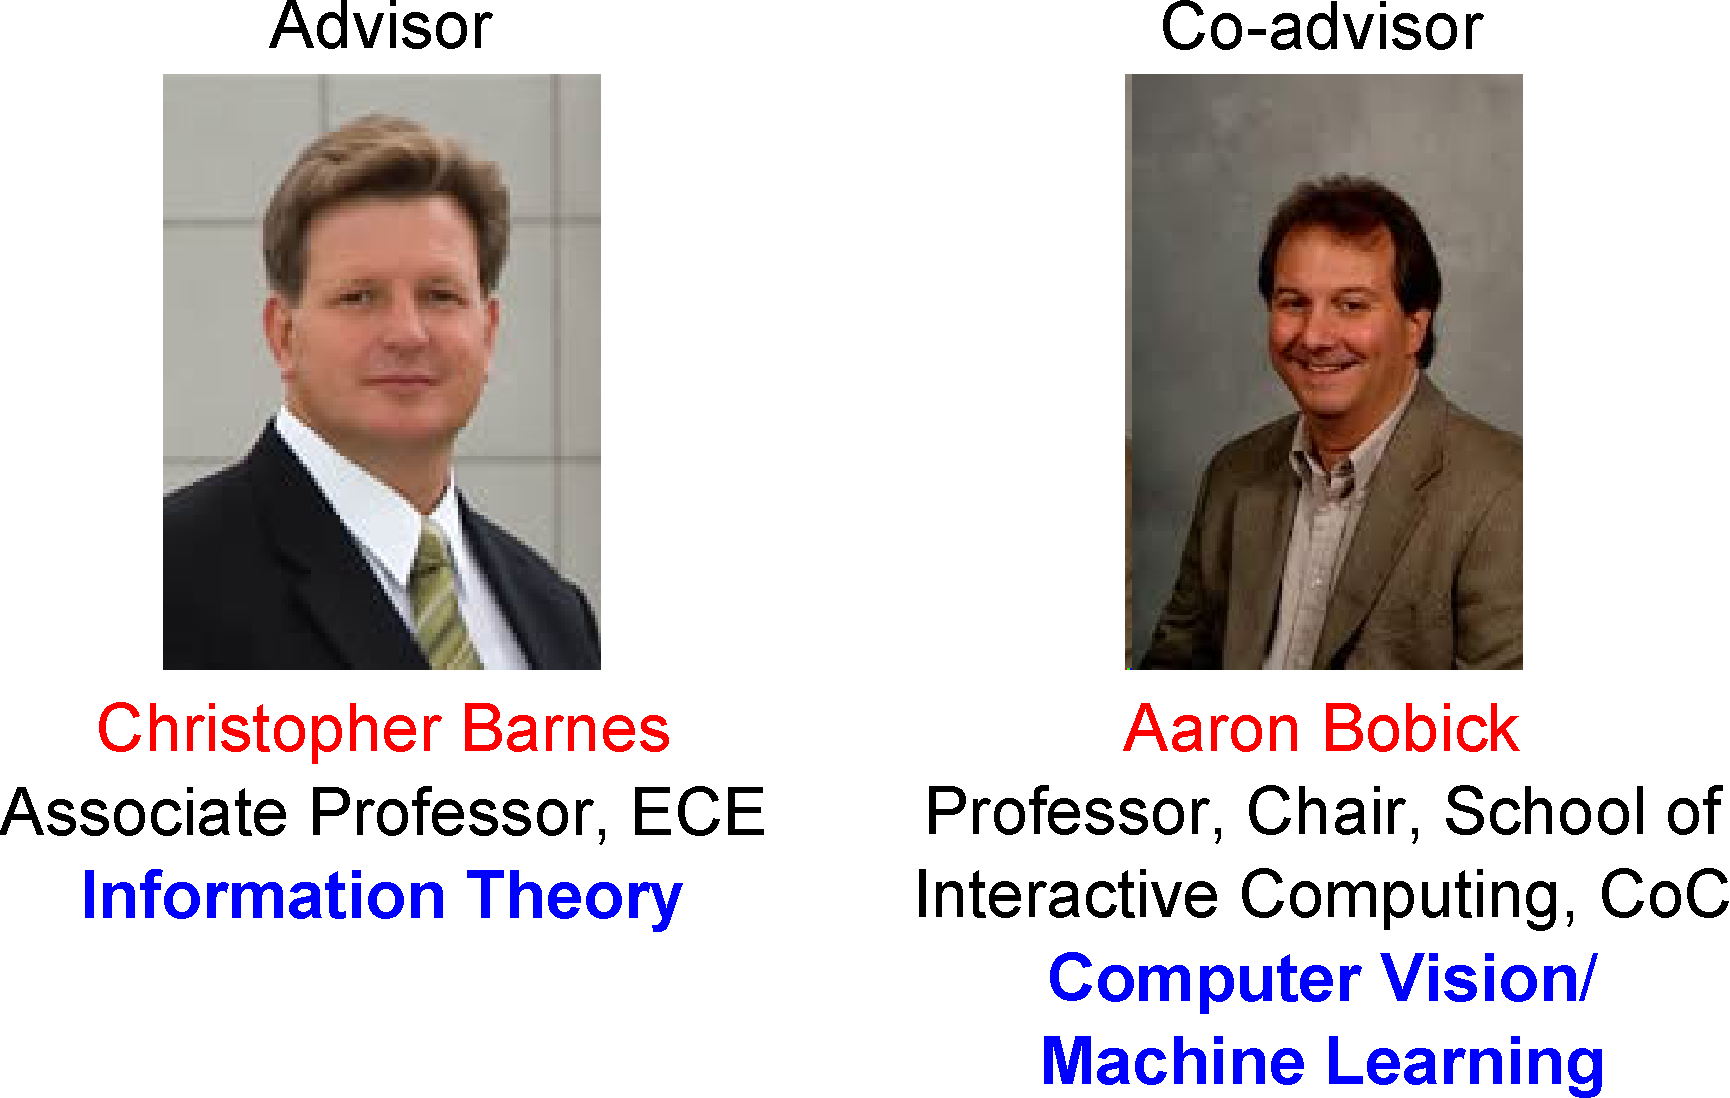
\includegraphics[width=0.73\textwidth]{thesis/professors.pdf}
\end{figure}
\end{frame}

%==================================
\section{II. Tracking}
%==================================
%---------------------------------------------------------
\subsection{(a) Introduction}
%---------------------------------------------------------
\begin{frame}
\frametitle{Tracking}
\framesubtitle{definition}
\logoCSIPCPL\mypagenum
	Estimate and maintain {\color{red}target state} over {\color{red}time}
	\begin{figure}
		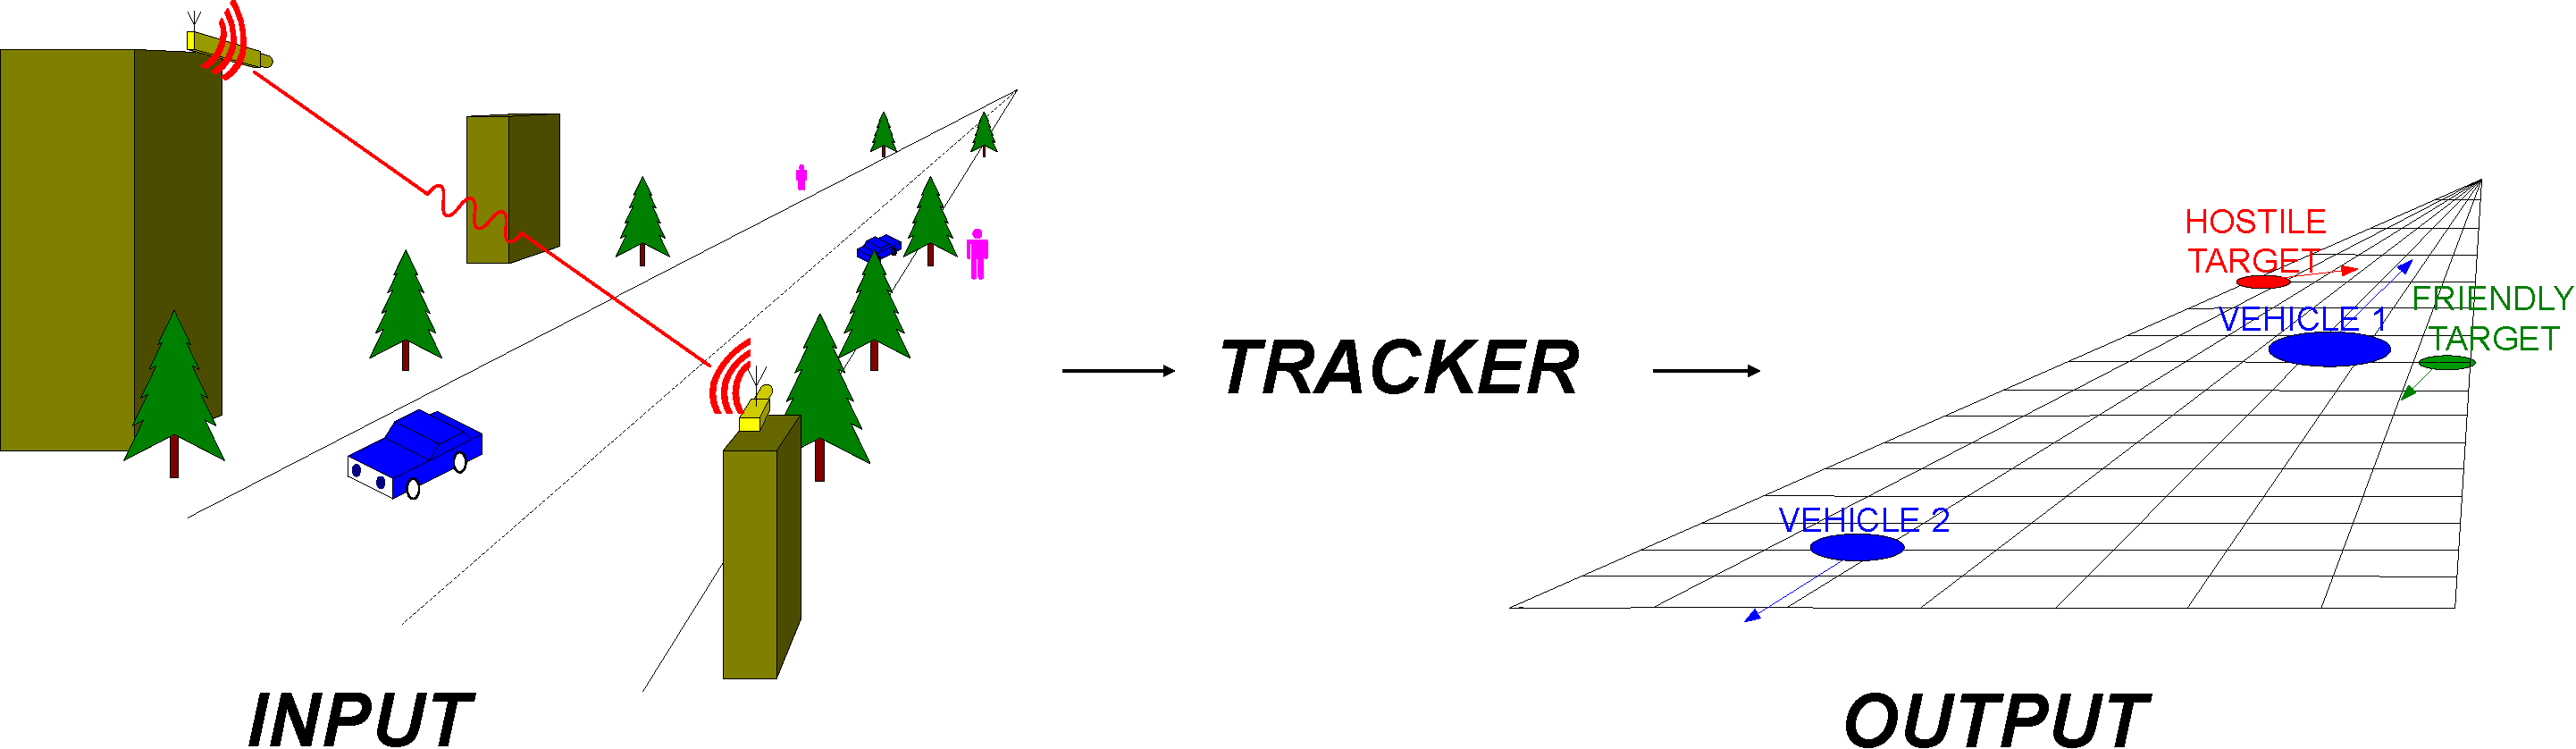
\includegraphics[width=1.0\textwidth]{thesis/TRK_overviewDiagram.pdf}
	\end{figure}
	\vspace{0.2in}
	2 step process
	\begin{itemize}
	\item Prediction: predict states using model
	\item Update: correction applied to prediction after observation arrives
	\end{itemize}
\end{frame}



\begin{frame}
\frametitle{Tracking}
\framesubtitle{Step 1 of 2: prediction (Chapman Kolmogorov)}
\logoCSIPCPL\mypagenum
\begin{table}
\begin{tabular}{|l|l|}\hline
$x_k$ & state at time $k$\\\hline
$Z_{k-1}$ &  all observations till time $k-1$\\\hline
\end{tabular}
\end{table}
\begin{figure}
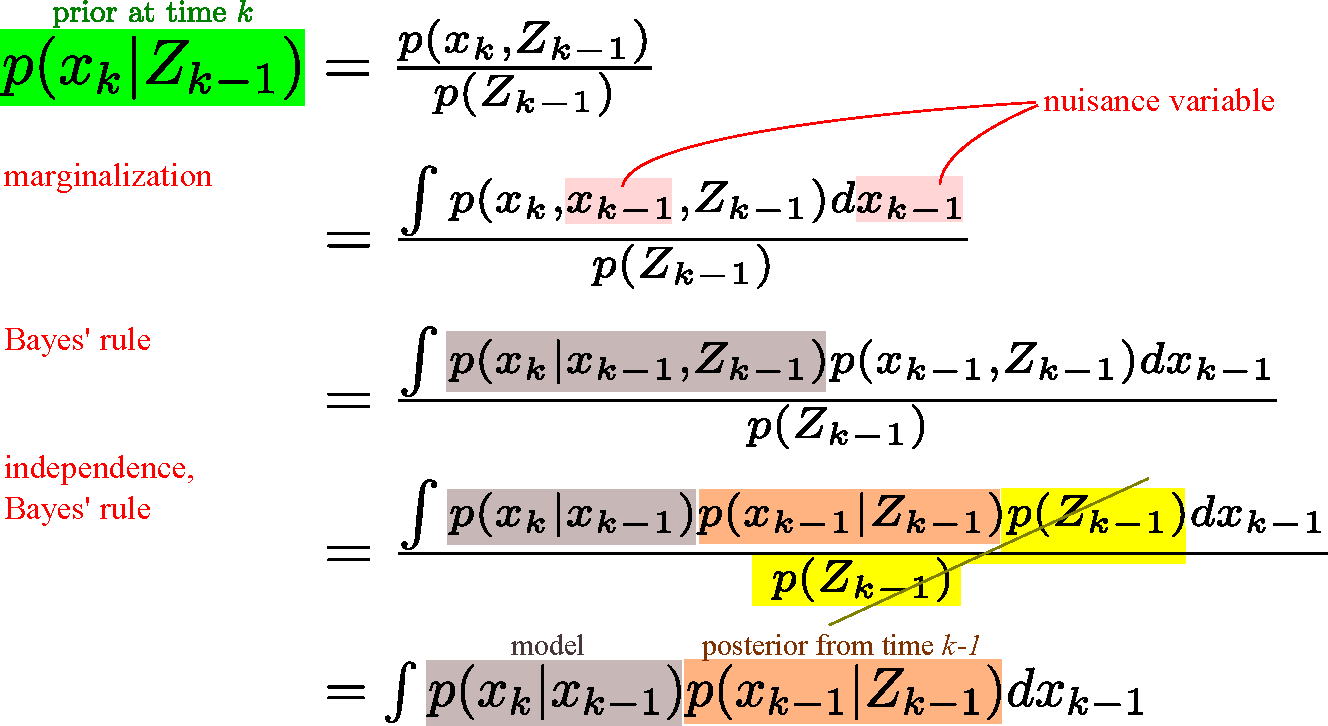
\includegraphics[width=1.0\textwidth]{thesis/TRK_EQN_prediction.pdf}
\end{figure}
\end{frame}


\begin{frame}
\frametitle{Tracking}
\framesubtitle{Step 2 of 2: update}
\logoCSIPCPL\mypagenum
\begin{figure}
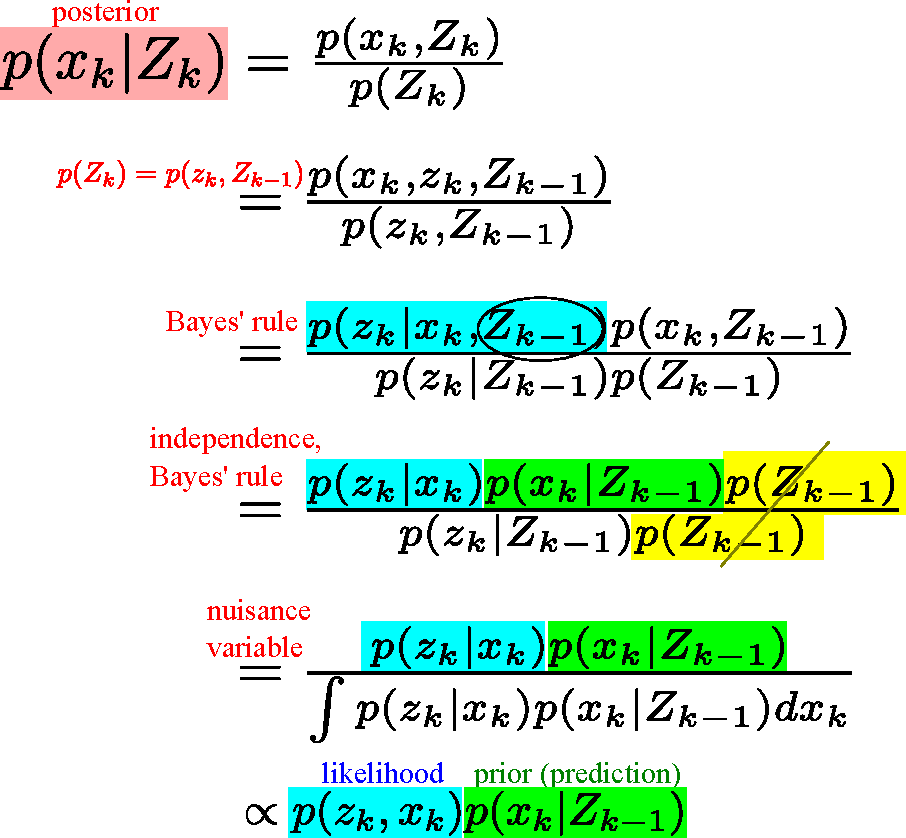
\includegraphics[height=0.8\textheight]{thesis/TRK_EQN_update.pdf}
\end{figure}
\end{frame}

\begin{frame}
\frametitle{Tracking}
\framesubtitle{Example: 1D tracking with particle filter}
\logoCSIPCPL\mypagenum
\begin{figure}
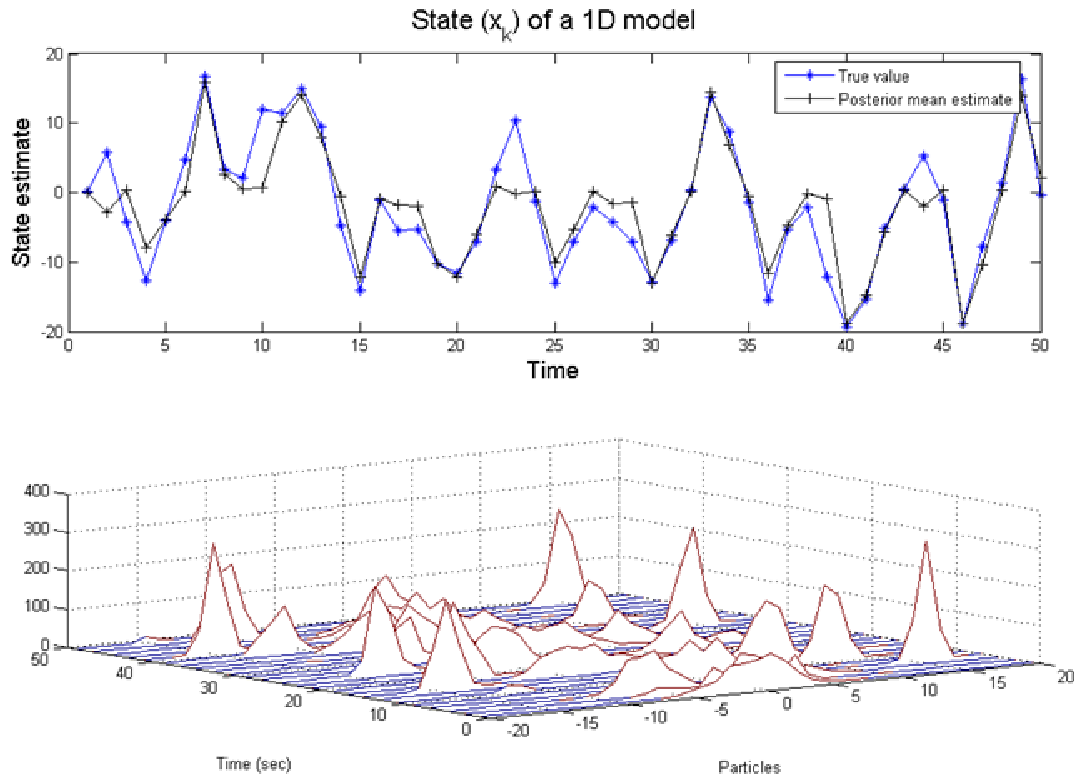
\includegraphics[width=1.0\textwidth]{thesis/TRK_ParticleFilter_multimodalPDF.pdf}
\end{figure}	
\end{frame}



\begin{frame}
\frametitle{Tracking}
\framesubtitle{probabilistic graphical models}
\logoCSIPCPL\mypagenum
	\begin{figure}
		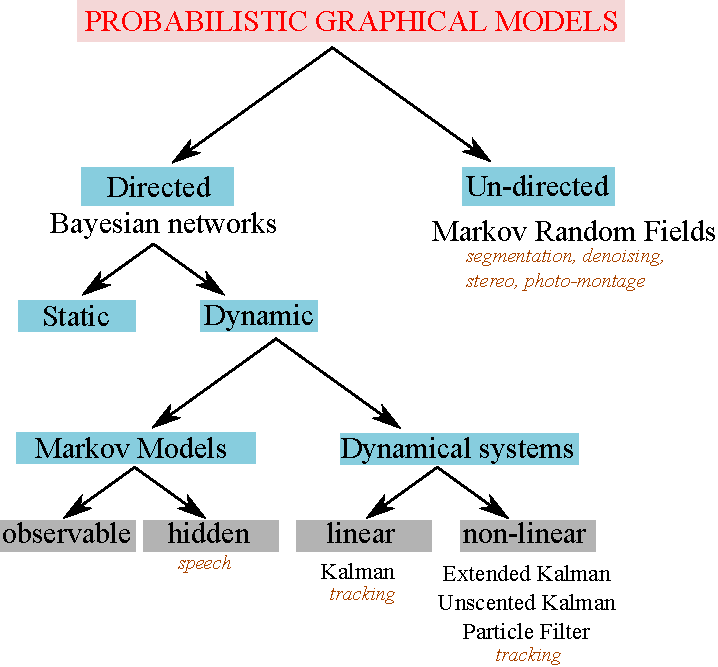
\includegraphics[width=0.9\textwidth]{thesis/PRML_PGM_overview.pdf}
	\end{figure}
\end{frame}


%---------------------------------------------------------
\subsection{(b) Computer vision}
%---------------------------------------------------------

\begin{frame}
\frametitle{Visual tracking}
\framesubtitle{components\tiny{\footnote {Yilmaz et.al., 2006}}}
\logoCSIPCPL\mypagenum
\begin{figure}
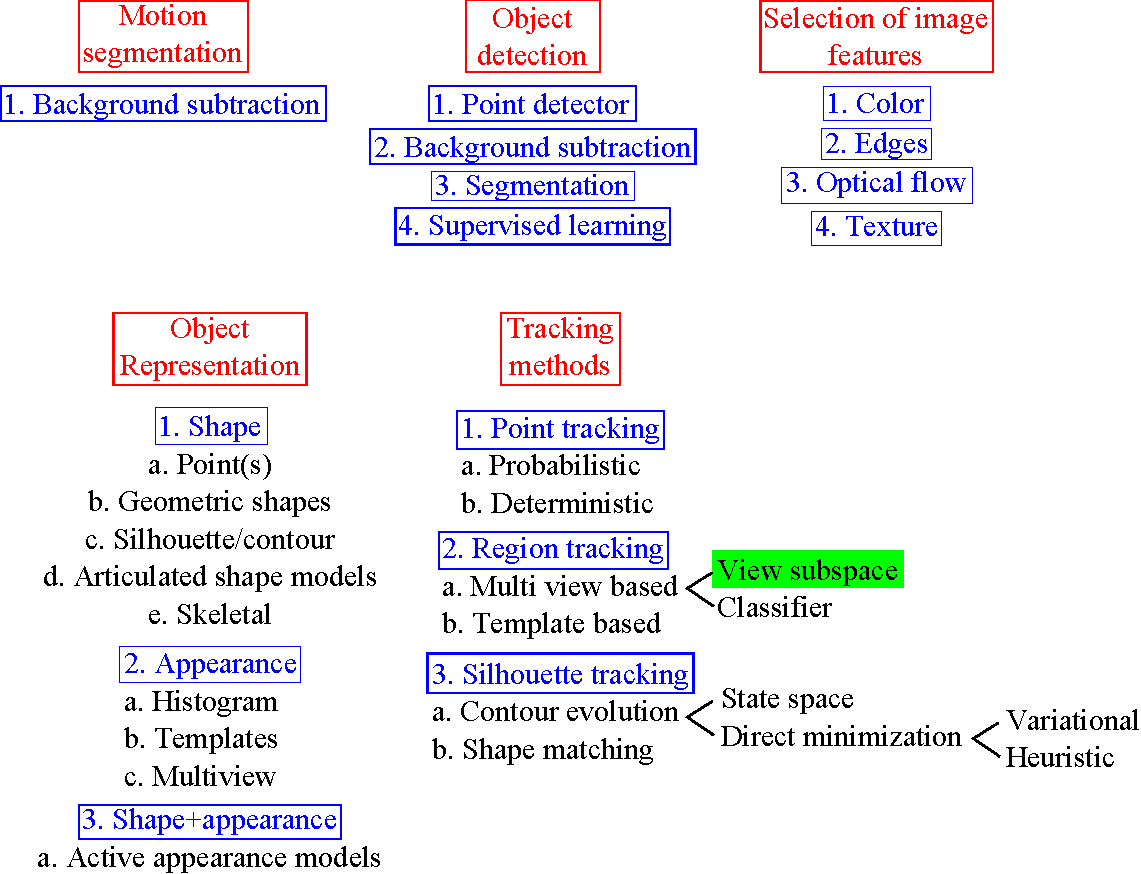
\includegraphics[height=0.8\textheight]{thesis/TRK_overview.pdf}
\end{figure}	
\end{frame}


\begin{frame}
\frametitle{Target representations\footnote{Yilmaz, 2006}}
\framesubtitle{}
\logoCSIPCPL\mypagenum
\begin{figure}[t]
\center
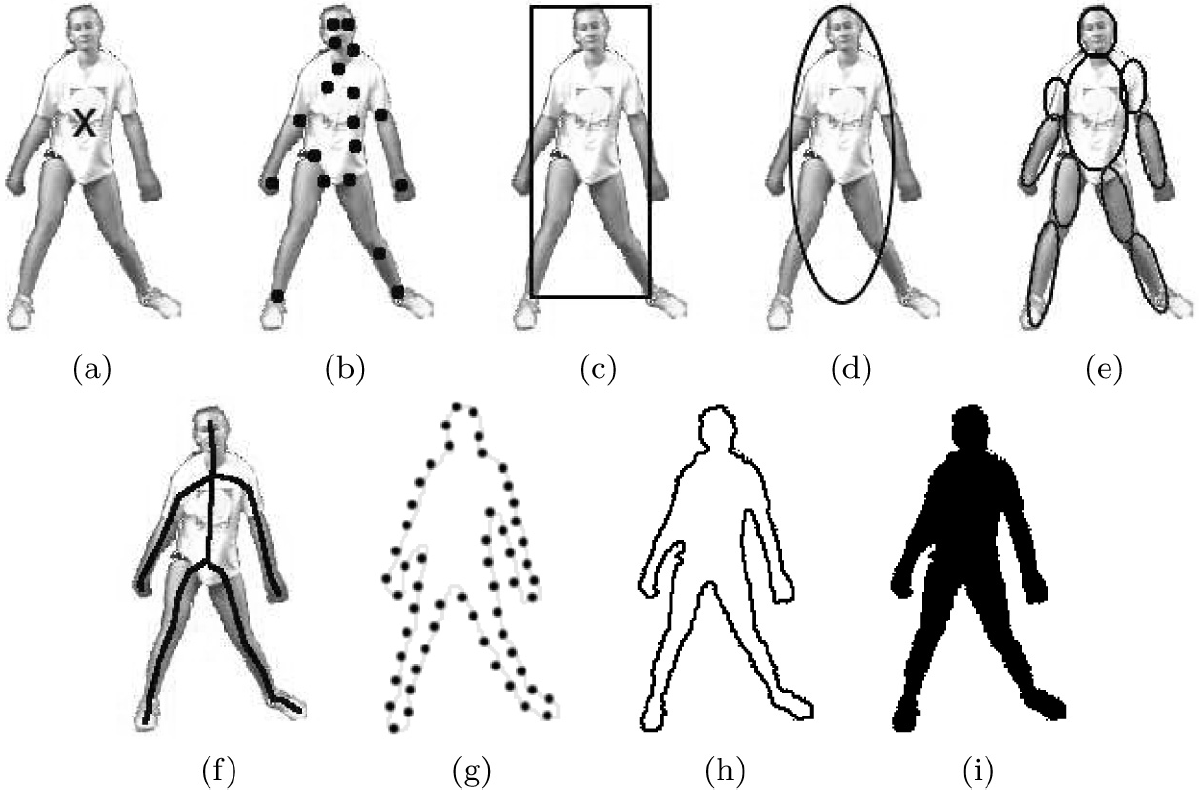
\includegraphics[width=0.8\textwidth]{thesis/2006_JNL_TRKsurvey_Shah_fig1.png}
\caption{Target representations.  (a) Centroid, (b) multiple points,(c) rectangular bounding box, (d) elliptical bounding region, (e) articulated shape model, (f) skeleton, (g) contour control points, (h) contour, (i) silhouette \cite{2006_JNL_SURVEYtrk_Yilmaz}.}
\label{fig:TRK_objectRepresentations}
\end{figure}
\end{frame}


\begin{frame}
\frametitle{Region tracking}
\framesubtitle{overview}
\logoCSIPCPL\mypagenum
	\begin{enumerate}
		\item Template matching
			\begin{itemize}
				\item simple
				\item fixed templates: reliable over short durations 
			\end{itemize}
		\item Subspace methods
			\begin{itemize}
				\item usually learned with PCA
				\item model variations in lighting and pose
				\item training data required
			\end{itemize}			
		\item Probability density
			\begin{itemize}
				\item robustness under image distortions and occlusions
				\item fast to learn
				\item registration can be difficult
			\end{itemize}
		\item Motion
			\begin{itemize}
				\item optical flow works well for small displacements
				\item block matching for large motion
				\item computing motion vectors is computationally complex
			\end{itemize}
	\end{enumerate}
\end{frame}




\begin{frame}
\frametitle{Region tracking}
\framesubtitle{Subspace tracking: prior work}
\logoCSIPCPL\mypagenum
\vspace{0.1in}
1998: first work on subspace tracking
	\begin{figure}
		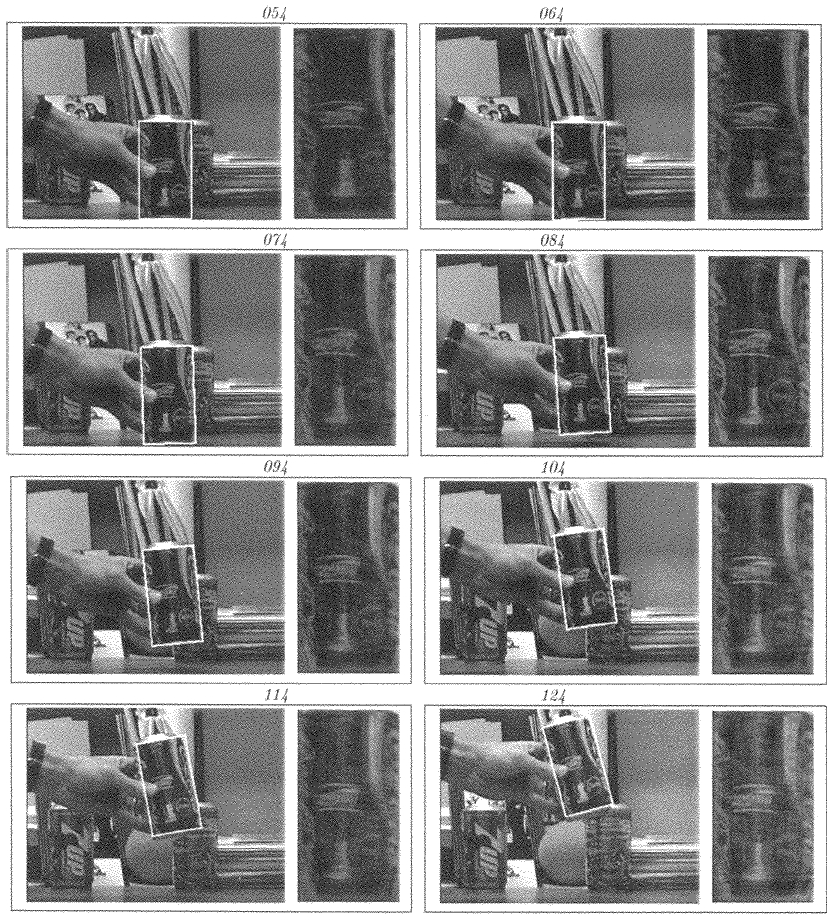
\includegraphics[width=0.6\textwidth]{thesis/TrackingPapers_SubspaceTracking_1998_Black_fig9.png}
	\end{figure}
\myFootnoteCitation{1998_JNL_Eigentracking_Black}{IJCV}
\end{frame}



\begin{frame}
\frametitle{Region tracking}
\framesubtitle{Subspace tracking: prior work}
\logoCSIPCPL\mypagenum
\vspace{0.1in}
2008: 10 years later, state of the art in subspace tracking
\begin{figure}
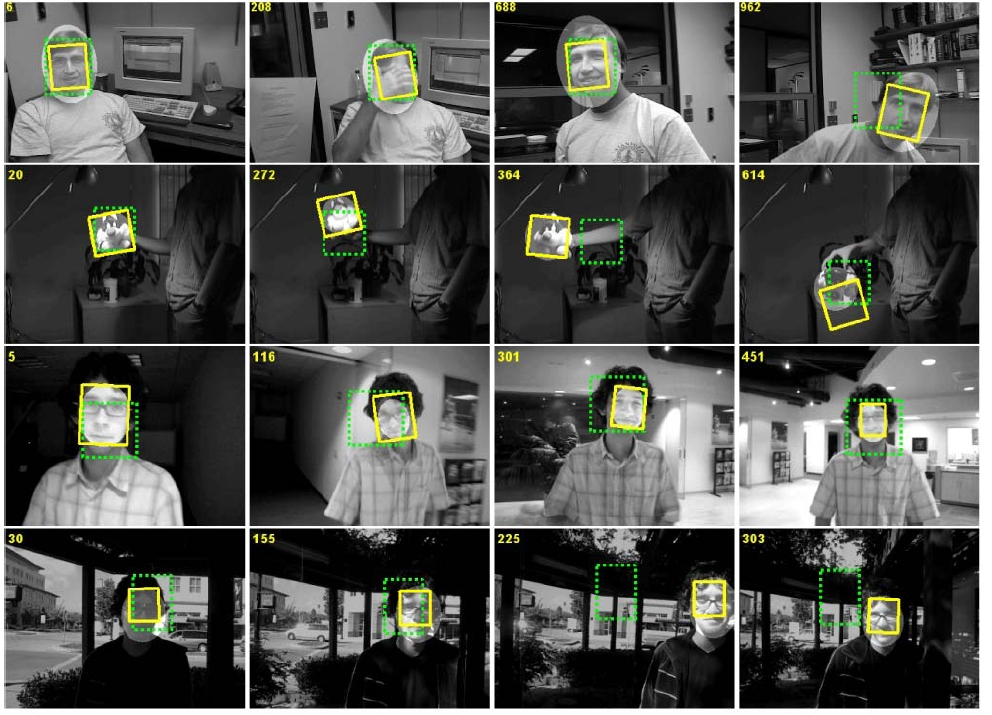
\includegraphics[width=0.9\textwidth]{thesis/TrackingPapers_SubspaceTracking_2008_Ross_fig10.png}
\end{figure}
\myFootnoteCitation{2008_JNL_subspaceTRK_Ross}{IJCV}
\end{frame}






%%---------------------------------------------------------
%\subsection{(b) Radars}
%%---------------------------------------------------------
%\begin{frame}
%\frametitle{Originally: radars}
%\framesubtitle{Kalman Filter}
%\logoCSIPCPL\mypagenum
%\begin{figure}
%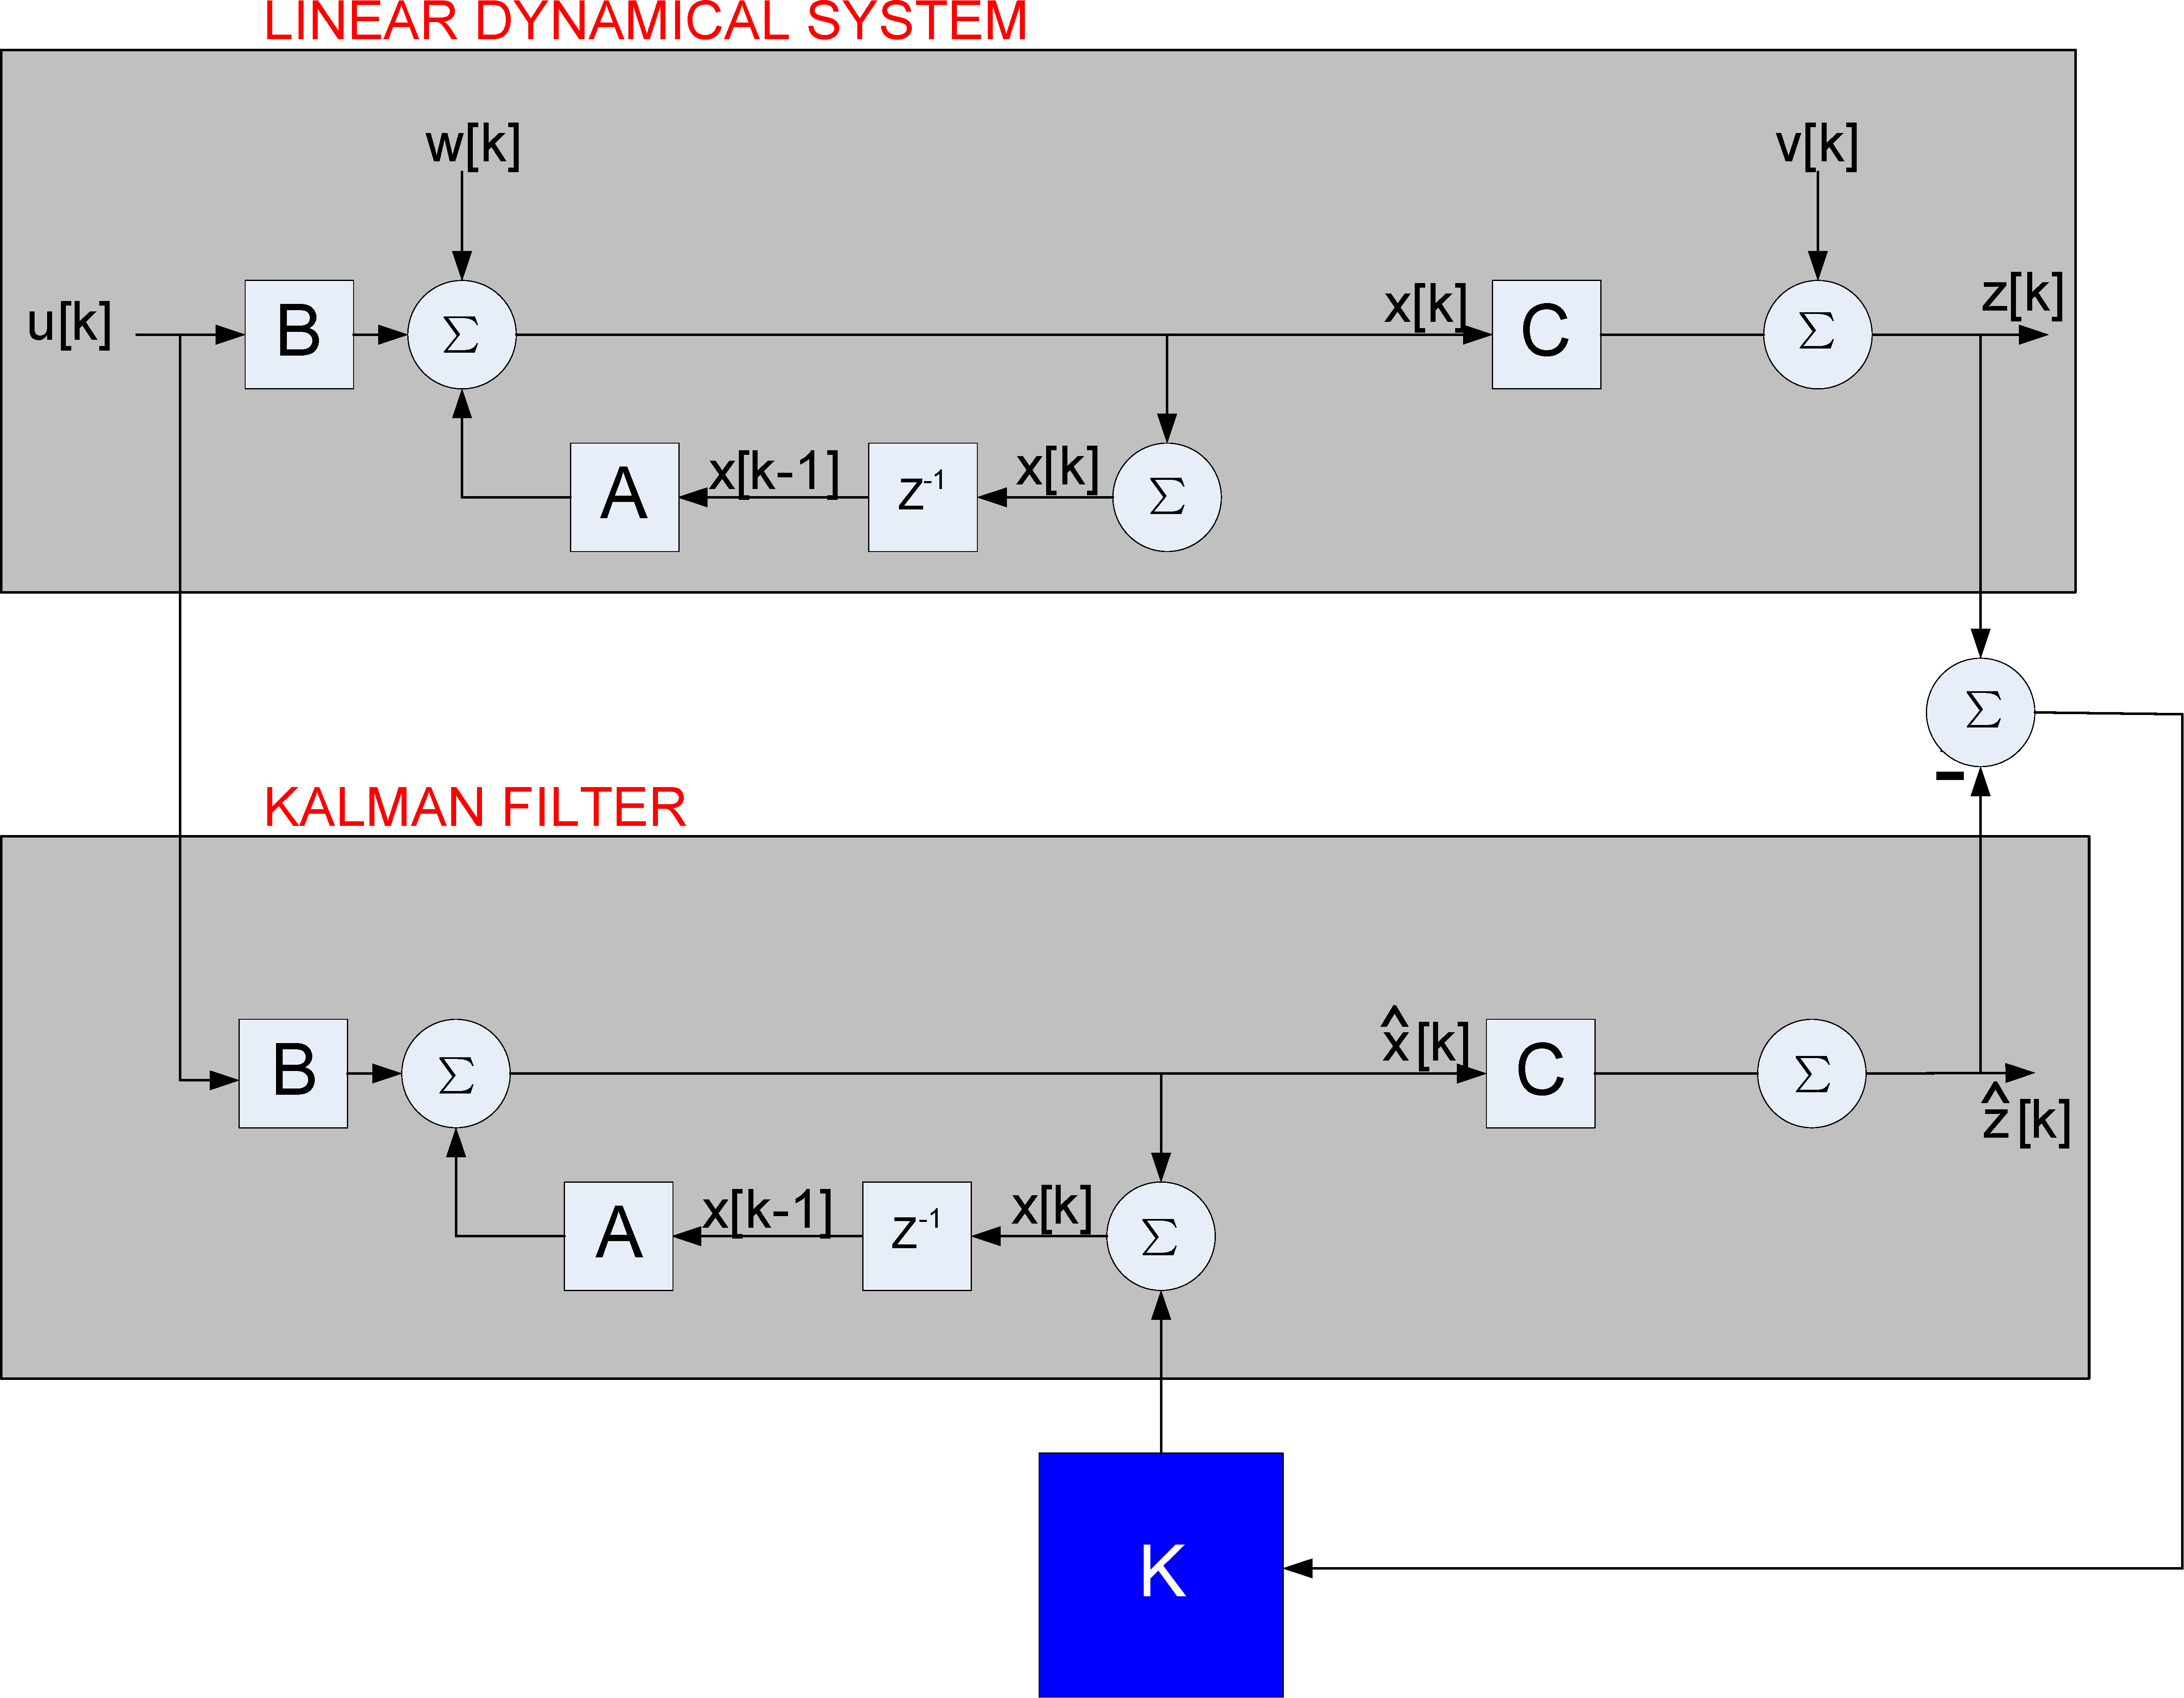
\includegraphics[width=1.0\textwidth]{thesis/TRK_KalmanFilter_blockDiagram.pdf}
%\end{figure}
%\end{frame}
%
%
%
%\begin{frame}
%\frametitle{Radar tracking\footnote{Bar-Shalom et al., 2009}}
%\framesubtitle{}
%\logoCSIPCPL\mypagenum
%\setcounter{subfigure}{0}
%\begin{figure}
%\subfigure[US Navy, long-range surveillance]{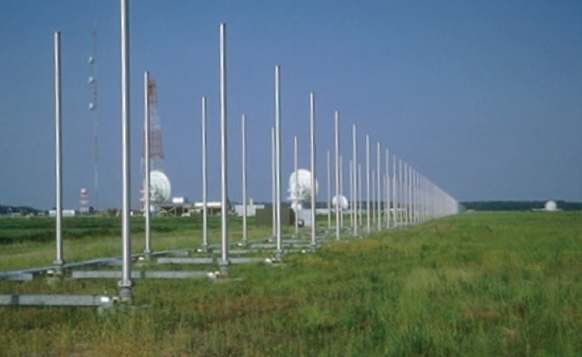
\includegraphics[height=0.2\textheight]{thesis/TRK_PDAF_example_US_Navy_ROTHR.png}}\hspace{0.2in}
%\subfigure[Theater High Altitude Area Defense]{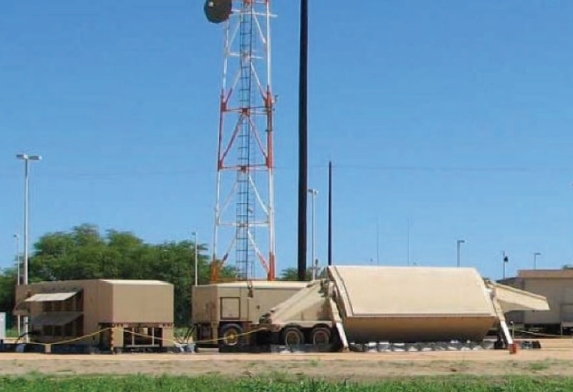
\includegraphics[height=0.2\textheight]{thesis/TRK_JPDAF_example_THAAD.png}}
%\subfigure[long-range surveillance against ICBMs]{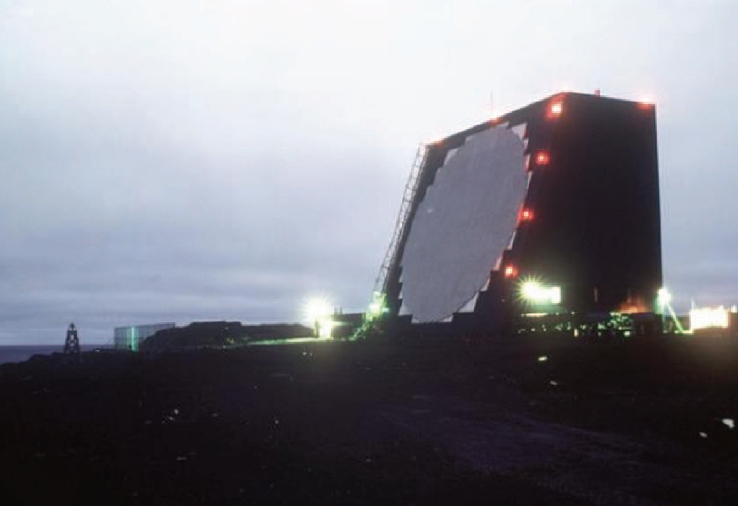
\includegraphics[height=0.2\textheight]{thesis/TRK_JPDAF_example_Cobra.png}}\hspace{0.2in}
%\subfigure[long-range surveillance against ICBMs]{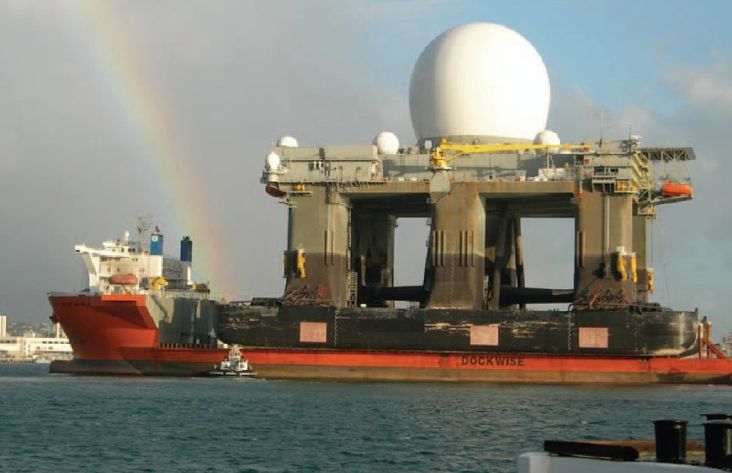
\includegraphics[height=0.2\textheight]{thesis/TRK_JPDAF_example_SBX.png}}
%\end{figure}
%\end{frame}








%\begin{frame}
%\frametitle{Pre-processing}
%\logoCSIPCPL\mypagenum
%	{\color{red}Steps}
%	\begin{enumerate}
%		\item Downsampling
%		\item Normalization
%		\item Stabilization
%		\item Background modeling
%		\item Feature Extraction
%	\end{enumerate}
%	\vspace{0.1in}
%	{\color{red}Features}
%	\begin{enumerate}
%		\item Color
%		\item Edges
%		\item Corners
%		\item Motion
%		\item Texture
%		\item Depth
%		\item Density
%	\end{enumerate}
%\end{frame}













%####################################################################################################
\section{III. RVQ}
%####################################################################################################
%--------------------------------------
\subsection{(a) Introduction}
%--------------------------------------
\begin{frame}
\frametitle{Quantization}
\framesubtitle{design-time}
\logoCSIPCPL\mypagenum
\begin{figure}				
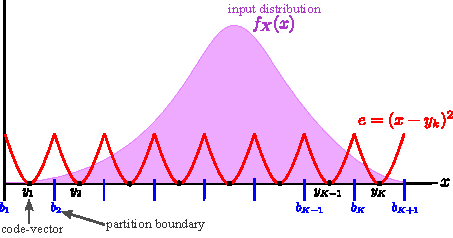
\includegraphics[width=1.0\textwidth]{thesis/Quantization_design_time.pdf}
\end{figure}
minimize distortion objective function
\begin{equation*}
e=\sum\limits_{k=1}^{K} \int\limits_{b_k}^{b_{k+1}}(x-y_k)^2f_X(x)
\end{equation*}
\end{frame}




\begin{frame}
\frametitle{Quantization}
\framesubtitle{design-time optimality: Lloyd Max conditions}
\logoCSIPCPL\mypagenum
\begin{figure}				
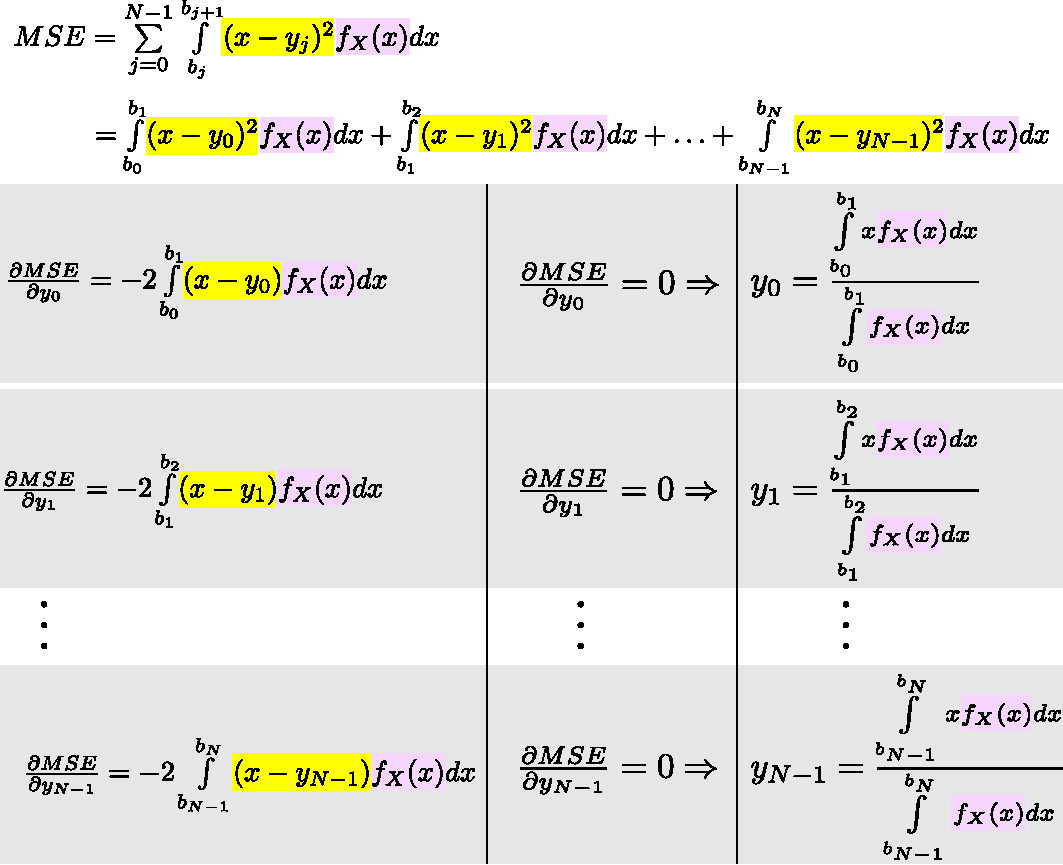
\includegraphics[height=0.75\textheight]{thesis/Quantization_optimalCodevectors.pdf}
\end{figure}
\end{frame}


\begin{frame}
\frametitle{Quantization}
\framesubtitle{run-time}
\logoCSIPCPL\mypagenum
\begin{itemize}
\item Quantizer $\mathcal{Q}$ maps input $\mathbf{x}_i$ to code-vector $\mathbf{y}_k$
\end{itemize}
\begin{figure}				
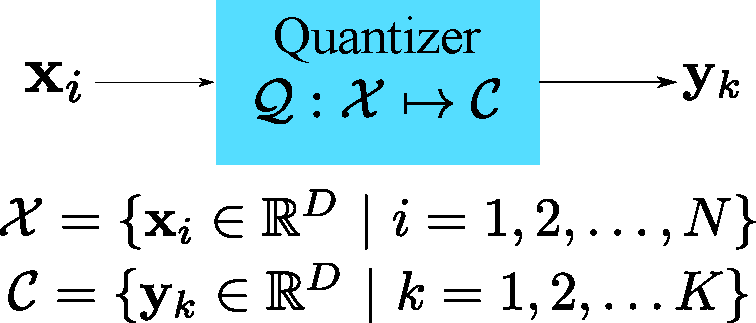
\includegraphics[width=0.9\textwidth]{thesis/Quantization_blockDiagram.pdf}
\end{figure}
\end{frame}




\begin{frame}
\frametitle{Vector Quantization}
\framesubtitle{types and advantages}
\logoCSIPCPL\mypagenum
	\begin{enumerate}
		\item Unstructured VQ
			\begin{itemize}
				\item Exhaustive Search (ESVQ)
			\end{itemize}
		\item Structured VQ
		\begin{itemize}
			\item Tree Structured (TSVQ)
			\item Transform
			\item Product
				\begin{itemize}
					\item Mean-removed
					\item Shape-gain
					\item Residual (RVQ)
				\end{itemize}
		\end{itemize}
	\end{enumerate}
	\vspace{0.2in}
	Makhoul, 1985 showed,
	\begin{itemize}
	\item decorrelation through rotation
	\item code-vector placement to take advantage of non-linear dependency
	\item cell-shape to take advantage of higher dimensionality
	\end{itemize}
\end{frame}


\begin{frame}
\frametitle{RVQ}
\framesubtitle{introduction}
\logoCSIPCPL\mypagenum
\begin{itemize}
\item $M$: number of code-vectors per stage
\item $P$: number of stages
\item pick one code-vector from each stage and add
\item $K=M^P$ possible such direct-sum additions
\item $K$ equivalent code-vectors, $y_k$
\item $y_k = \mu_1^{(k)} + \mu_2^{(k)} + \ldots + \mu_P^{(k)}$
\end{itemize}
\begin{figure}[t]
\centering
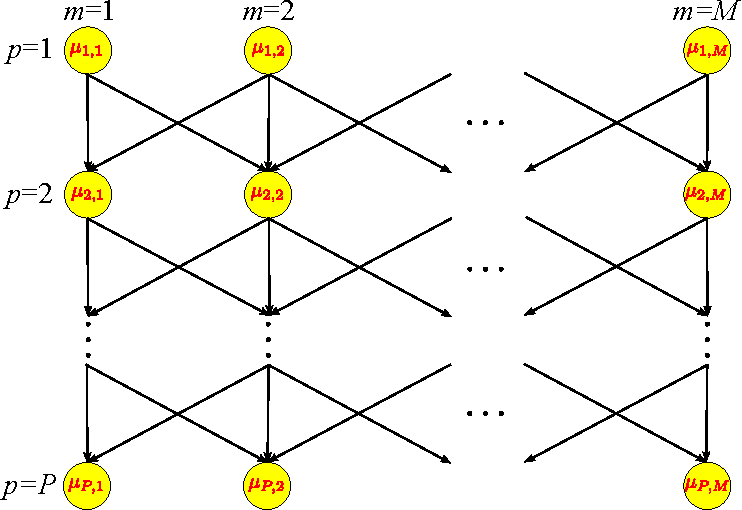
\includegraphics[width=0.7\textwidth]{thesis/RVQ.pdf}
\end{figure}
\end{frame}


\begin{frame}
\frametitle{RVQ}
\framesubtitle{introduction: example, equivalent code-vectors}
\logoCSIPCPL\mypagenum
\begin{figure}[t]
\centering
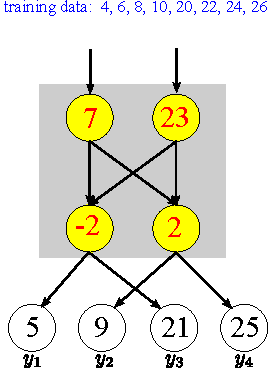
\includegraphics[width=0.5\textwidth]{thesis/RVQ_introduction.pdf}
\end{figure}
\end{frame}


%--------------------------------------
\subsection{(b) Design-time}
%--------------------------------
\begin{frame}
\frametitle{RVQ}
\framesubtitle{design-time}
\logoCSIPCPL\mypagenum
\begin{itemize}
\item $x_i$: input data point
\item $\mu_\rho^{(k)}$: stage code-vector at $\rho$-th stage that maps to $k$-th equivalent code-vector, $y_k$
\end{itemize}
\scriptsize
\begin{align}
e &= \KmeansError\notag\\
&= \KmeansSum{\bigg[\RVQmultipleKmeansone\bigg]}^2, \ \ \rho=1\notag\\
&= \KmeansSum{\bigg[\RVQmultipleKmeanstwo\bigg]}^2, \ \ \rho=2\notag\\
&\ \ \ \  \ \ \ \vdots\notag\\
&=\KmeansSum{\bigg[\RVQmultipleKmeansT\bigg]}^2, \ \ \rho=P\notag
\end{align}
\end{frame}


\begin{frame}
\frametitle{RVQ}
\framesubtitle{design-time (cont.)}
\logoCSIPCPL\mypagenum
\scriptsize
\begin{align*}
e	&= \KmeansSum{\bigg[\RVQmultipleKmeansonealternate\bigg]}^2, \ \ \rho=\{1, 2, \ldots P\}\notag\\
&={\RVQerroralternate}, \ \ \rho=\{1, 2, \ldots P\}
\end{align*}
\vspace{0.1in}
\normalsize
\begin{itemize}
\item $\mu_\rho^{(k)}$ can be computed using Lloyd Max conditions
\item This step is called the causal anti-causal (CAC) condition in Barnes, 1993
\item We call it a coupled K-means condition
\item $\mu_\rho^{(k)}$ is a causal anti-causal centroid
\end{itemize}
\end{frame}


\begin{frame}
\frametitle{RVQ}
\framesubtitle{design-time: sample 8x4 codebook}
\logoCSIPCPL\mypagenum
\setcounter{subfigure}{0}
\begin{figure}[h!]
\centering\subfigure{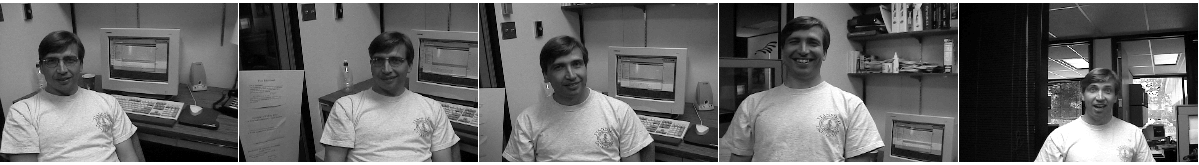
\includegraphics[height=0.41in]{thesis/seq_1_Dudek.png}\label{fig:trk_pca_1a}}
\subfigure{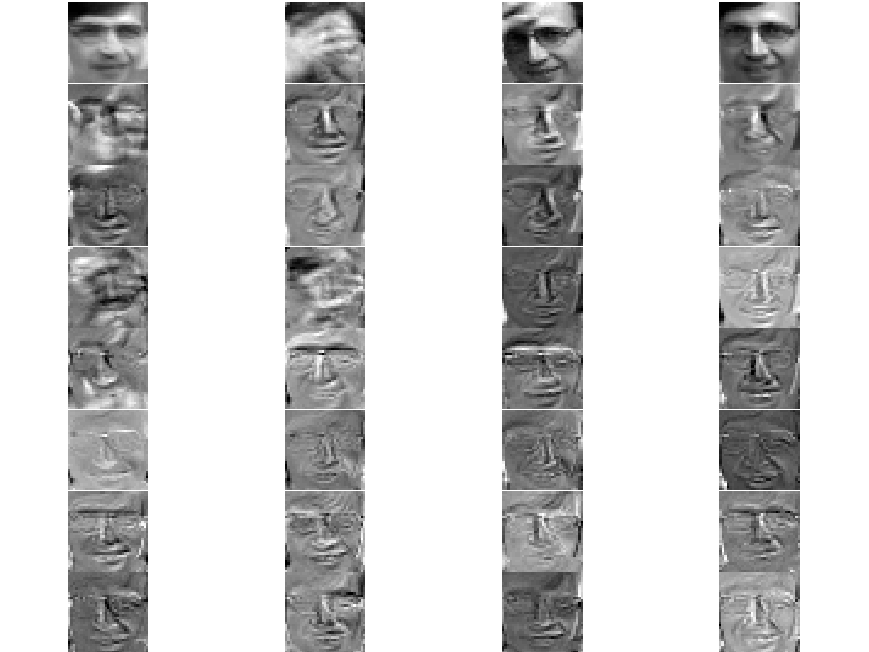
\includegraphics[height=0.65\textheight]{thesis/1_Dudek__aRVQ_08_04_1000_0_RofE__170_codebook.pdf}
}
\end{figure}
\end{frame}


%--------------------------------------
\subsection{(c) Run-time}
%--------------------------------------

\begin{frame}[plain]
\frametitle{RVQ}
\framesubtitle{run-time: block diagram}
\logoCSIPCPL\mypagenum
\begin{changemargin}{-1.35in}{0in}
\setcounter{subfigure}{0}
\begin{figure}
\centering			
\subfigure[Encoder.]{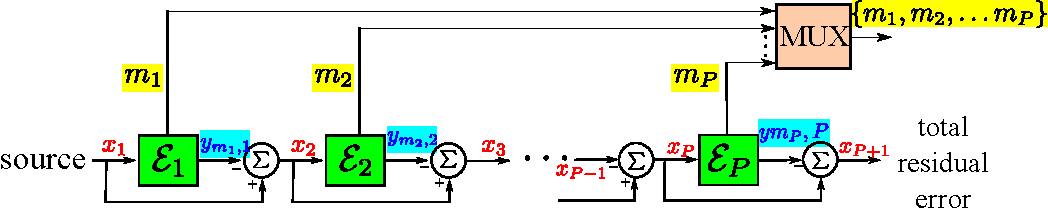
\includegraphics[width=1.35\textwidth]{thesis/RVQ_encoder_blockDiagram.pdf}}
\subfigure[Decoder.]{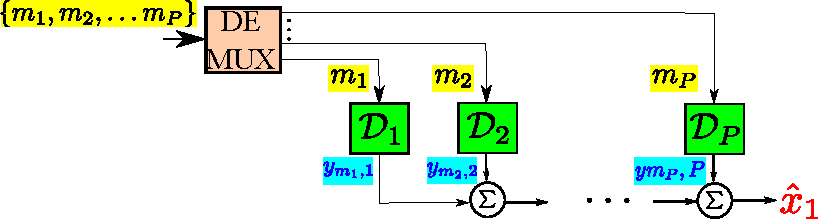
\includegraphics[width=1.15\textwidth]{thesis/RVQ_decoder_blockDiagram.pdf}}
\end{figure}
\end{changemargin}
\end{frame}


%\begin{frame}
%\frametitle{RVQ}
%\framesubtitle{distortion}
%\logoCSIPCPL\mypagenum
%	\begin{figure}				
%		\includegraphics[width=1.0\textwidth]{thesis/RVQ_distortion.pdf}
%	\end{figure}
%\end{frame}





\begin{frame}
\frametitle{RVQ}
\framesubtitle{run-time: example}
\logoCSIPCPL\mypagenum
\begin{itemize}
\item During design-time, 3x2 codebook generated from training data: $S$=\{1, 2, ... 7\}
\item reconstruction starts at 0
\end{itemize}
\begin{figure}[t]
\centering
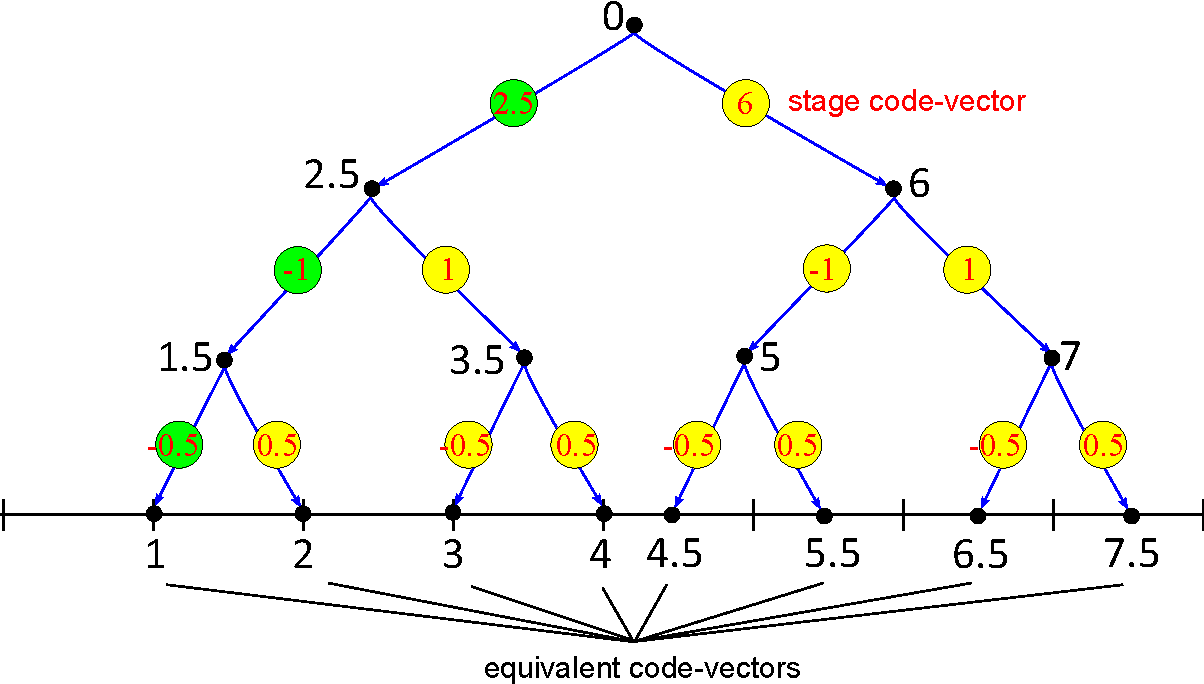
\includegraphics[width=0.9\textwidth]{thesis/RVQ_trg_1_to_7_equivalentCVs.pdf}
%\subfigure[Entanglement using a 2x4 encoder codebook.]{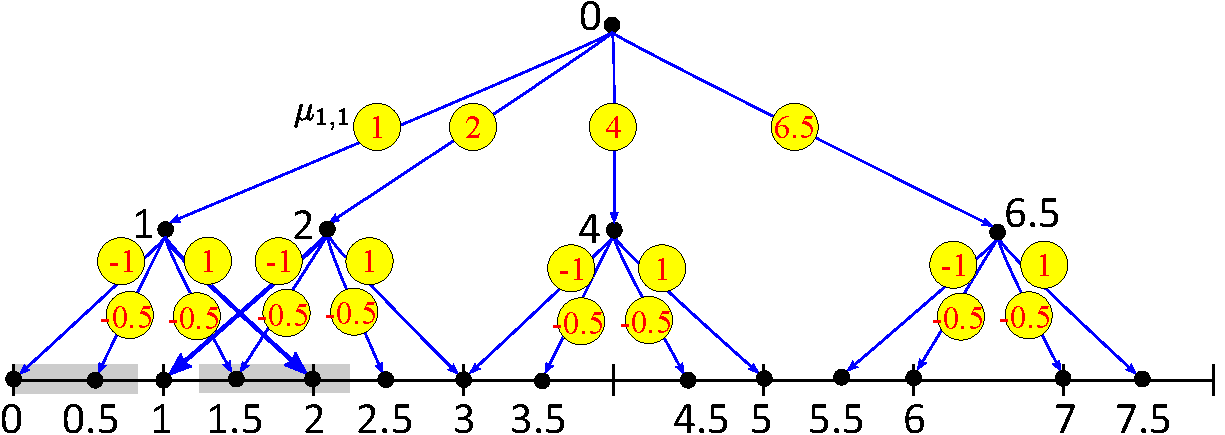
\includegraphics[width=0.75\textwidth]{thesis/RVQ_trg_1_to_7_equivalentCVs_2.pdf}}
\end{figure}
\end{frame}



\begin{frame}
\frametitle{RVQ}
\framesubtitle{run-time: 4 encoding methods}
\logoCSIPCPL\mypagenum
\begin{enumerate}
\item \underline{maxP}: In this method, RVQ decoding is carried out so that maximum stages $P$ are used.
\item \underline{RofE}: In this method, realm of experience coding is used.  In other words, a test vector is decoded such that the decode path traversed belongs to the set of training decode paths.
\item \underline{nulE}: In this method, null encoding is used.  Reconstruction rms error is checked at every stage.  If at any stage, rms error is not reduced, that stage is skipped.
\item \underline{monR}: In this method, monotonic rms error is a condition.  If this condition is not met, decoding stops.
\end{enumerate}
\end{frame}



\begin{frame}[plain]
\frametitle{RVQ}
\framesubtitle{run-time: 4 encoding methods, example}
\logoCSIPCPL\mypagenum
\begin{changemargin}{-1.3in}{0in}
\setcounter{subfigure}{0}
\begin{figure}[h]
\centering
\subfigure[reconstruct 8]{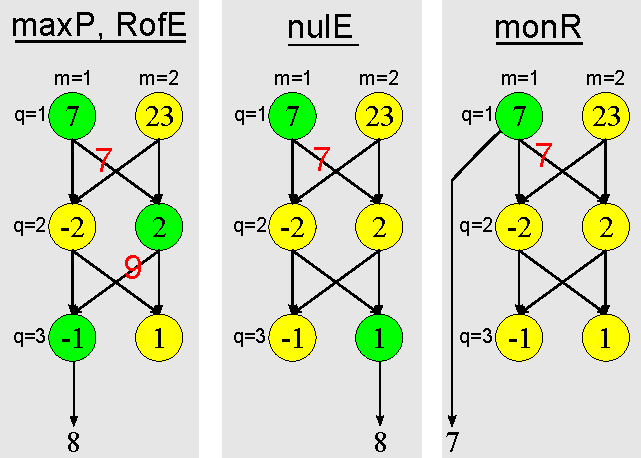
\includegraphics[width=0.6\textwidth]{thesis/RVQ_CAC_toyExample_3x2.pdf}}				\subfigure[reconstruct 13]{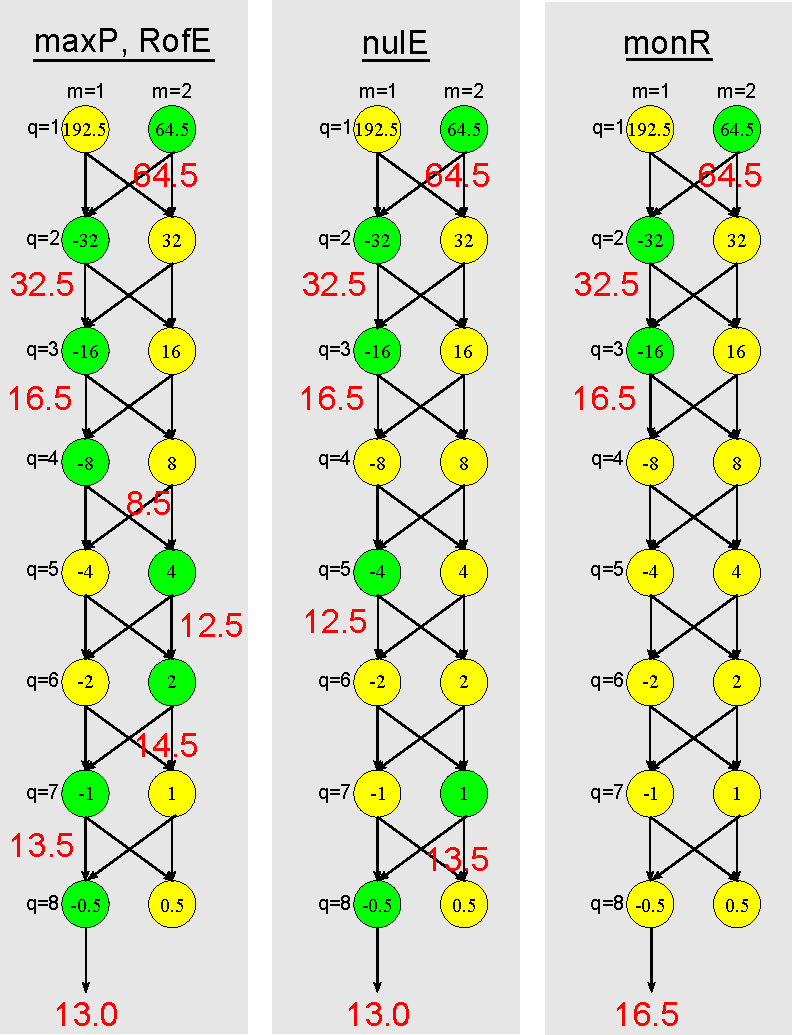
\includegraphics[width=0.6\textwidth]{thesis/RVQ_CAC_toyExample_8x2.pdf}}
\end{figure}
\end{changemargin}
\end{frame}


%--------------------------------------
\subsection{(d) Comparisons}
%--------------------------------------
\begin{frame}[plain]
\frametitle{Comparison with ESVQ, TSVQ}
\framesubtitle{}
\mypagenum
\begin{changemargin}{-1.3in}{0in}
\begin{figure}		
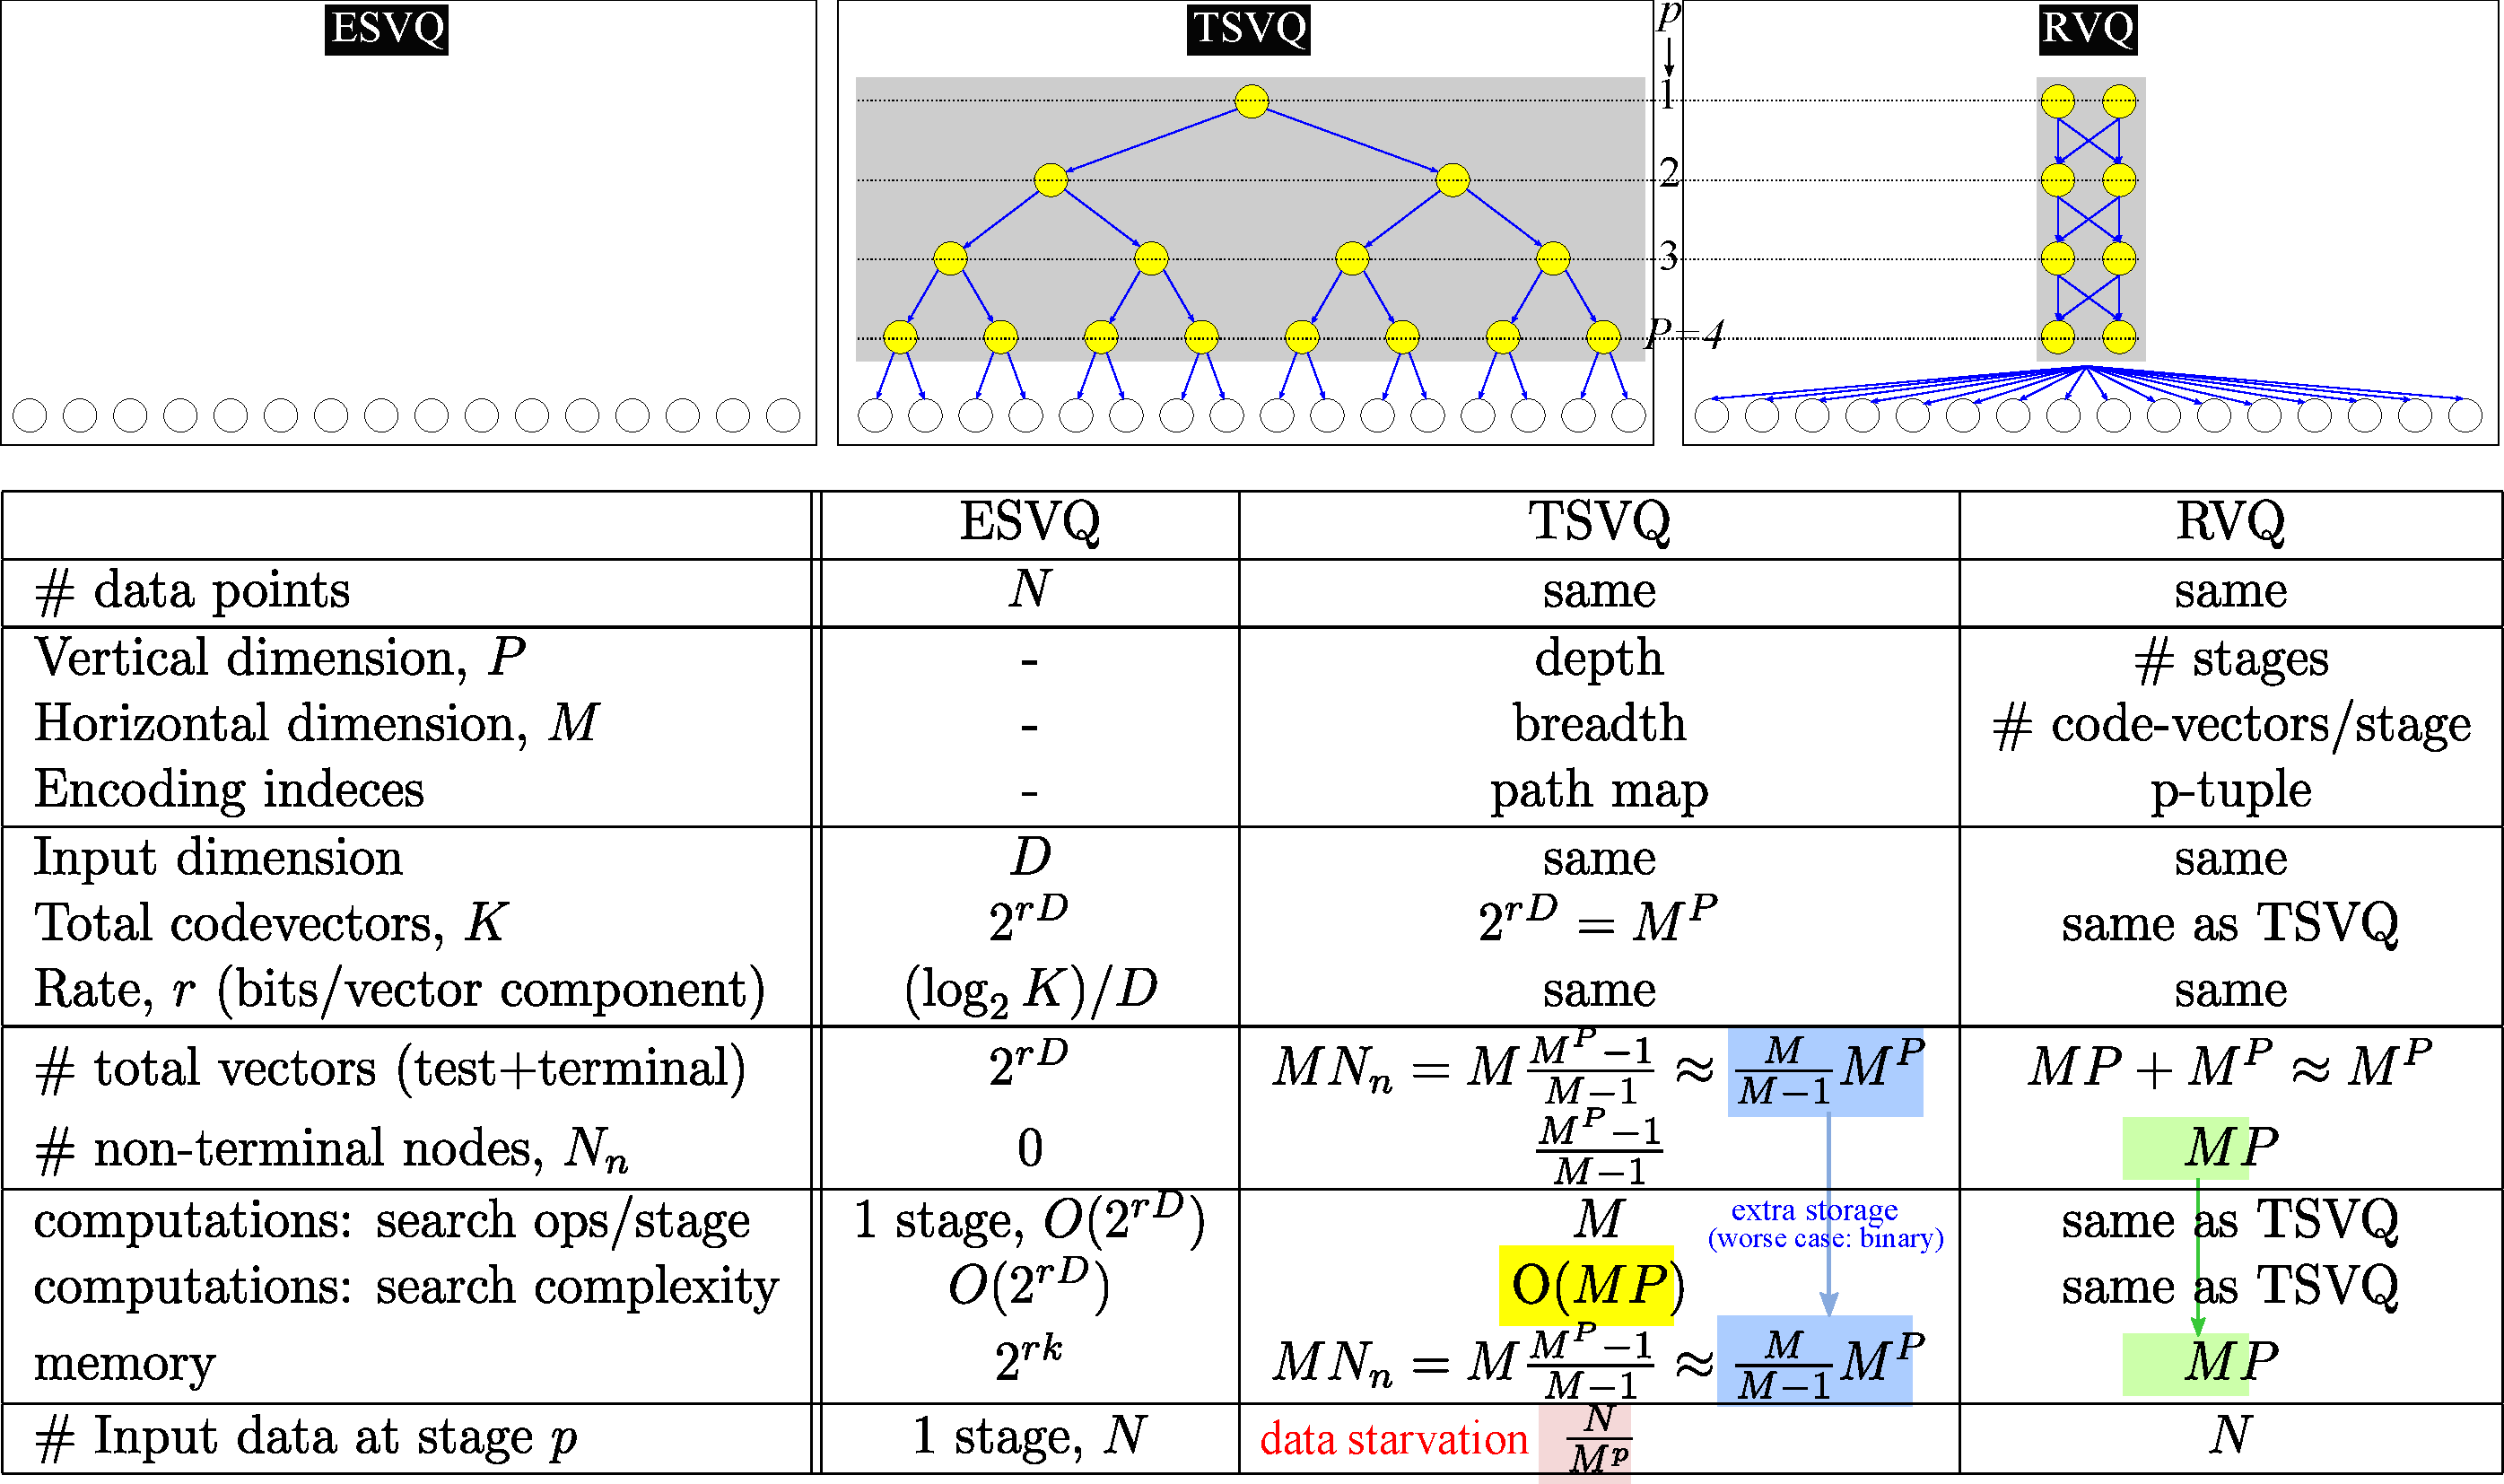
\includegraphics[width=1.3\textwidth]{thesis/RVQ_comparisonWithESVQ_TSVQ.pdf}			
\end{figure}
	Generally, structurally constrained quantizers cannot provide performance as good as ESVQ
	\begin{itemize}
		\item RVQ can handle higher dimensions due to linear complexity
		\item Better performance than ESVQ possible, for given implementation cost
	\end{itemize}	

\end{changemargin}
\end{frame}




\begin{frame}
\frametitle{Comparison with PCA}
\framesubtitle{}
\logoCSIPCPL\mypagenum
\begin{figure}		
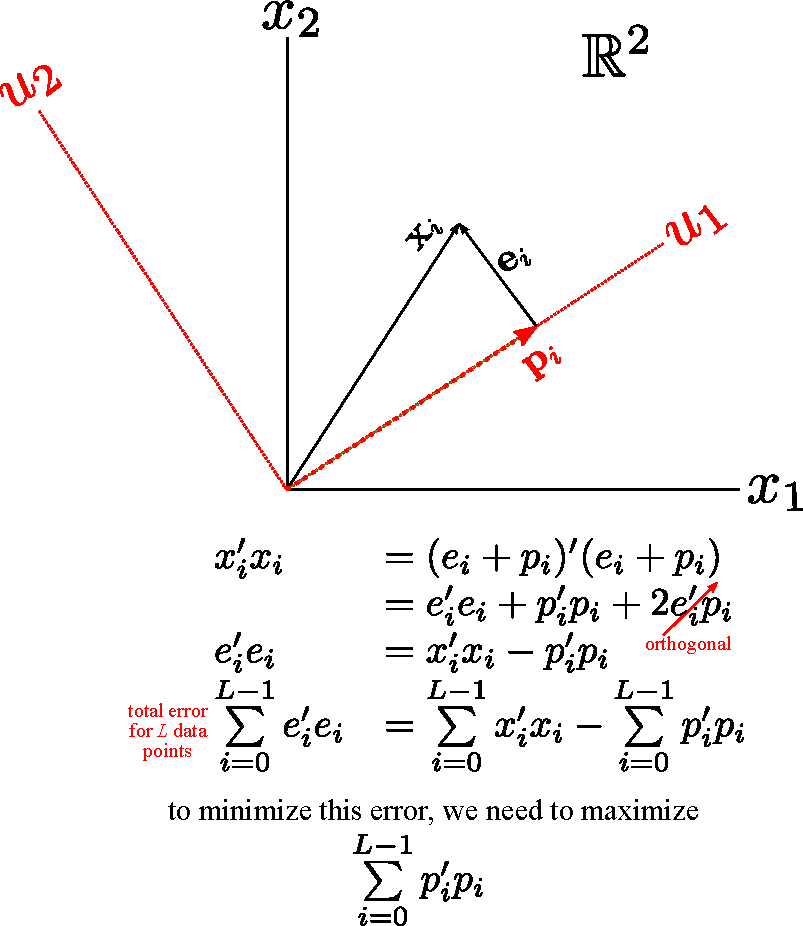
\includegraphics[width=0.6\textwidth]{thesis/PRML_PCA_geometricDerivation_step1.pdf}			
\end{figure}
\begin{itemize}
\item In PCA, goal is to minimize orthogonal distance to subspace
\item In VQ, goal is to minimize Euclidean distance to closest centroid
\end{itemize}
\end{frame}


%\begin{frame}[plain]
%\frametitle{RVQ comparison}
%\framesubtitle{2. with TSVQ}
%\logoCSIPCPL\mypagenum
%%	\begin{changemargin}{-1.3in}{0in}
%%		\begin{figure}				
%%			\includegraphics[width=1.3\textwidth]{thesis/RVQ_comparisonWithTSVQ.pdf}
%%		\end{figure}
%%	\end{changemargin}
%\end{frame}



%\begin{frame}[plain]
%\frametitle{RVQ comparison}
%\framesubtitle{3. with PCA}
%\logoCSIPCPL\mypagenum
%	\begin{changemargin}{-1.3in}{0in}
%		\begin{figure}				
%			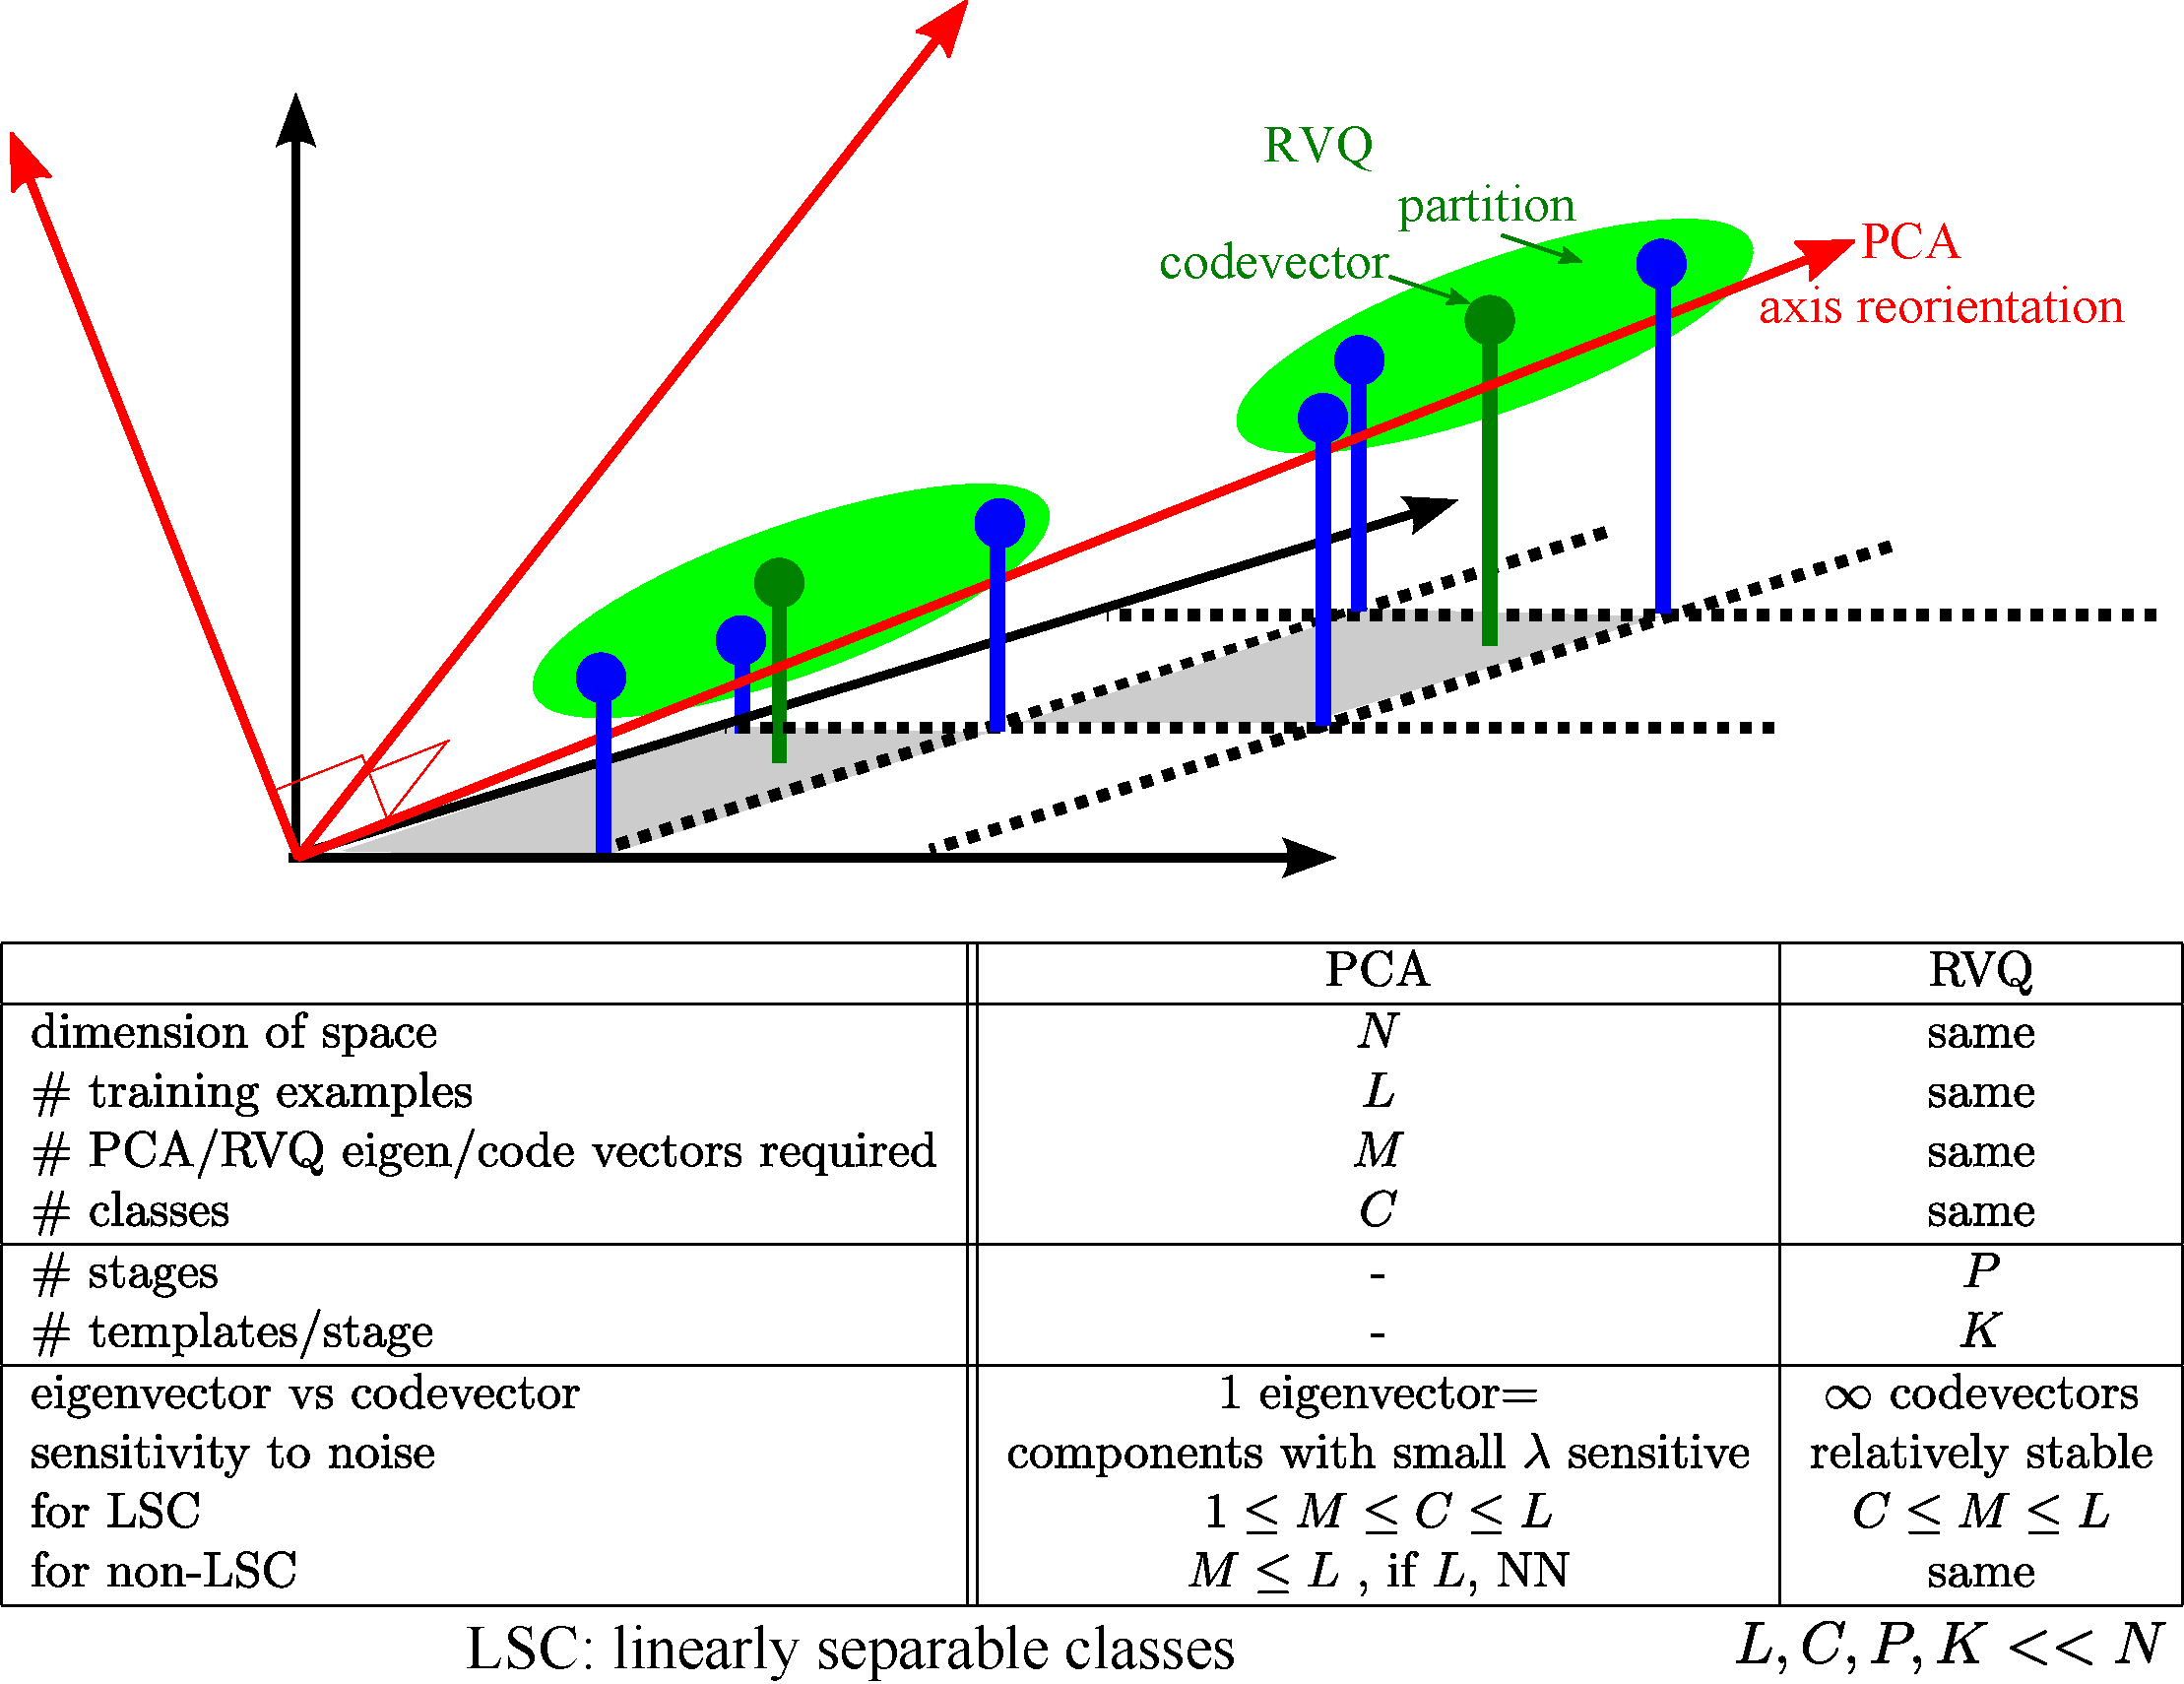
\includegraphics[width=1.3\textwidth]{thesis/RVQ_comparisonWithPCA.pdf}
%		\end{figure}
%	\end{changemargin}
%\end{frame}


%--------------------------------------------------------
\subsection{(e) Image classification}
%--------------------------------------------------------
\begin{frame}
\frametitle{Image classification\footnote{Barnes, 2007}}
\framesubtitle{\small Satellite imagery: pre-Tsunami Sri Lanka \\(training phase)}
\logoCSIPCPL\mypagenum
	\begin{figure}		
		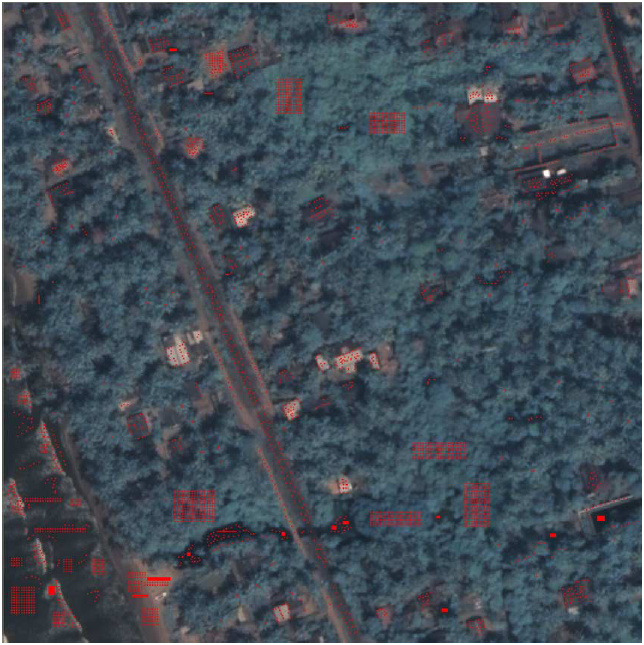
\includegraphics[height=0.3\textheight]{thesis/RVQ_SatelliteSriLanka_1_snippets.png}			
	\end{figure}
	\begin{figure}		
		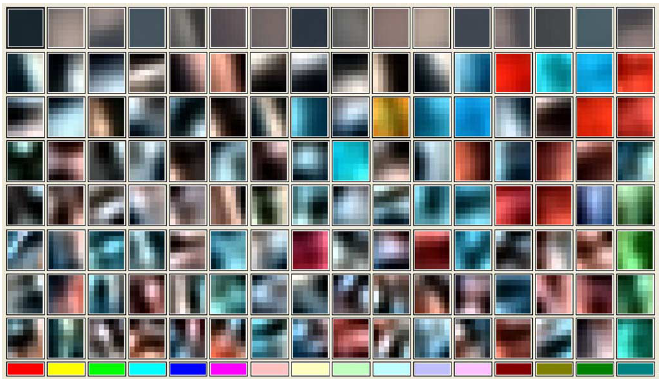
\includegraphics[height=0.35\textheight]{thesis/RVQ_SatelliteSriLanka_2_codebooks.png}			
	\end{figure}
\end{frame}




\begin{frame}
\frametitle{Image classification\footnote{Barnes, 2007}}
\framesubtitle{\small Satellite imagery: pre-Tsunami Sri Lanka\\(testing phase)}
\logoCSIPCPL\mypagenum
	\begin{figure}		
		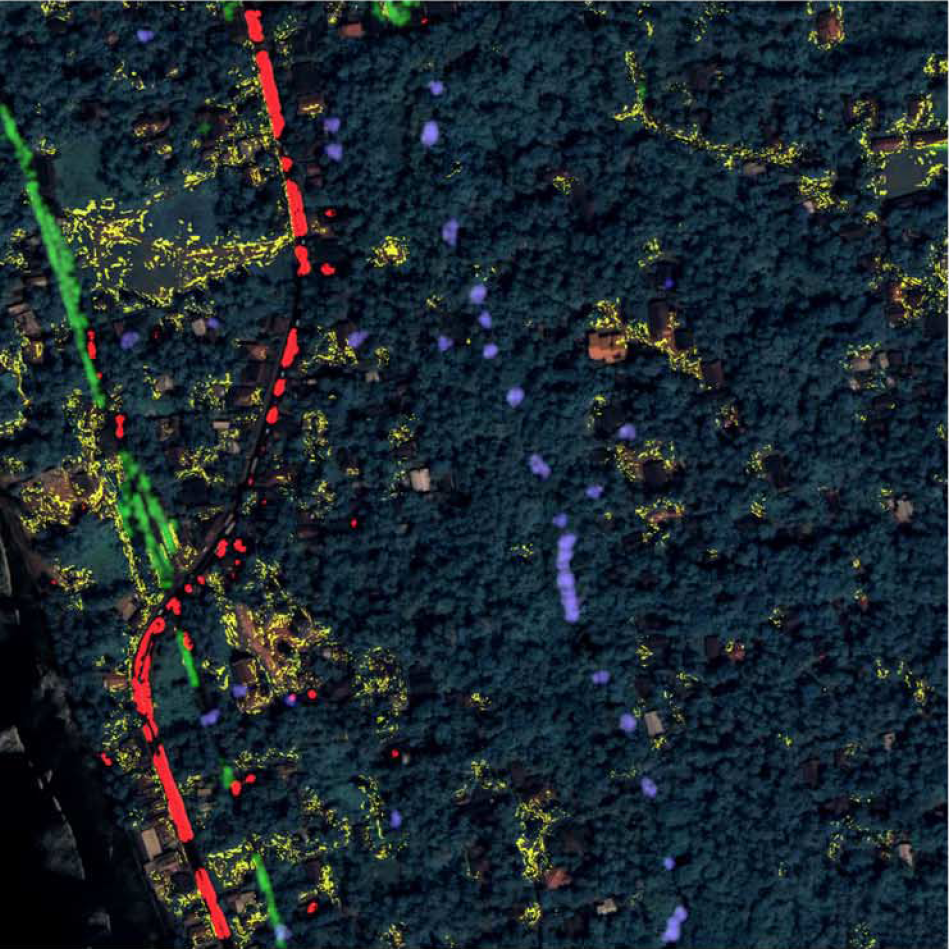
\includegraphics[height=0.5\textheight]{thesis/RVQ_SatelliteSriLanka_3_labeling.png}
		\caption{\hspace{1.3in}{\color{yellow}yellow}: dirt paths \\\hspace{1.3in}{\color{blue}blue}: rivers \\\hspace{1.3in}{\color{red}red}: paved roads \\\hspace{1.3in}{\color{green}green}: train tracks}
	\end{figure}
\end{frame}


%=======================================
\section{IV. RVQ tracking}
%=======================================
\begin{frame}
\frametitle{Experimental overview}
\framesubtitle{}
\logoCSIPCPL\mypagenum
\setcounter{subfigure}{0}
\begin{figure}[t]
\centering
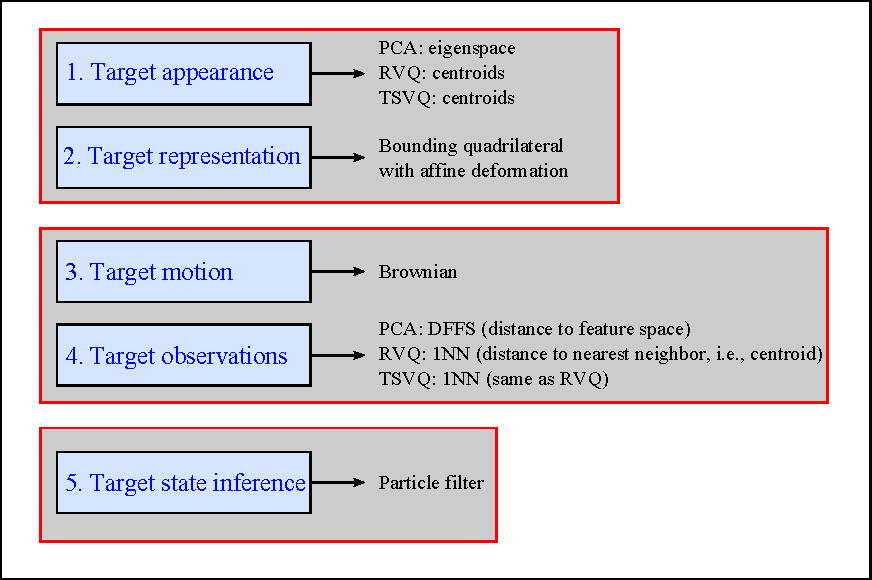
\includegraphics[width=1.0\textwidth]{thesis/PhD_experimentalOverview.pdf}
\label{fig:overview}
\end{figure}
\end{frame}



\begin{frame}[plain]
\frametitle{Temporal evolution}
\framesubtitle{}
\logoCSIPCPL\mypagenum
\setcounter{subfigure}{0}
\begin{changemargin}{-1.3in}{0in}
\begin{figure}[t]
\centering
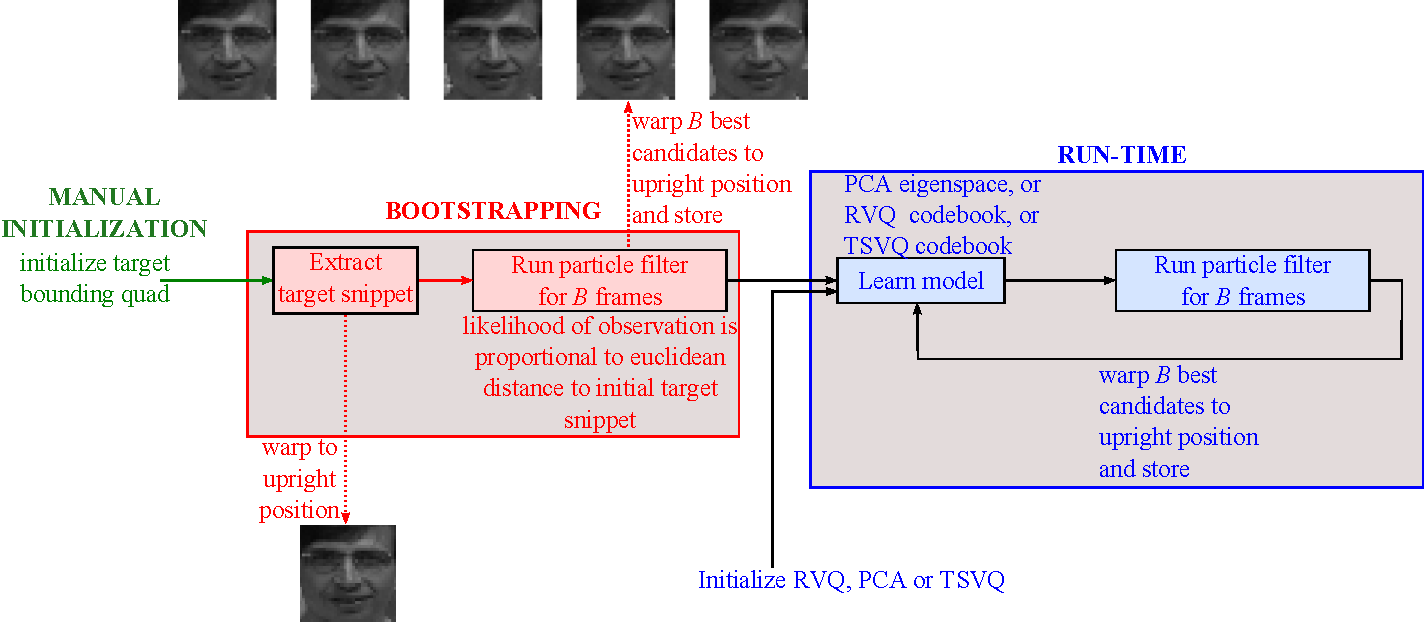
\includegraphics[width=1.3\textwidth]{thesis/PhD_experimentalTemporalOverview.pdf}
\label{fig:temporal_overview}
\end{figure}
\end{changemargin}
\end{frame}


\begin{frame}
\frametitle{Publicly available datasets\footnote{Ross et. al. 2008}}
\framesubtitle{Dudek, davidin300, sylv, fish, car4, car11}
\logoCSIPCPL\mypagenum
\setcounter{subfigure}{0}
\begin{figure}[h!]
\centering\subfigure{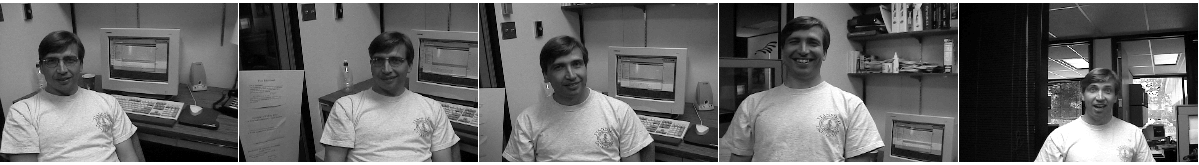
\includegraphics[height=0.41in]{thesis/seq_1_Dudek.png}\label{fig:trk_pca_1a}}
\subfigure{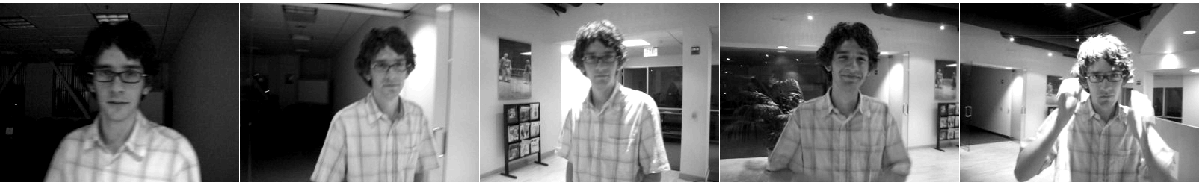
\includegraphics[height=0.41in]{thesis/seq_2_davidin300.png}\label{fig:trk_pca_1b}}
\subfigure{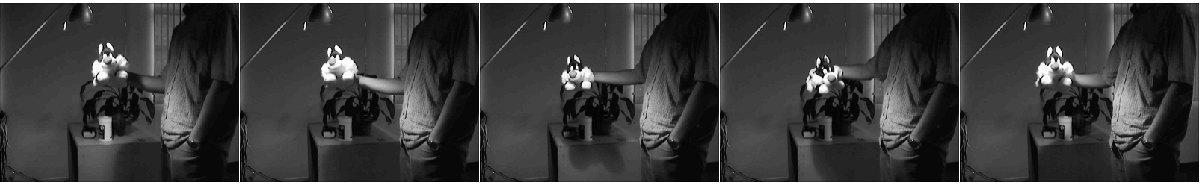
\includegraphics[height=0.41in]{thesis/seq_3_sylv.png}\label{fig:trk_pca_1c}}
\subfigure{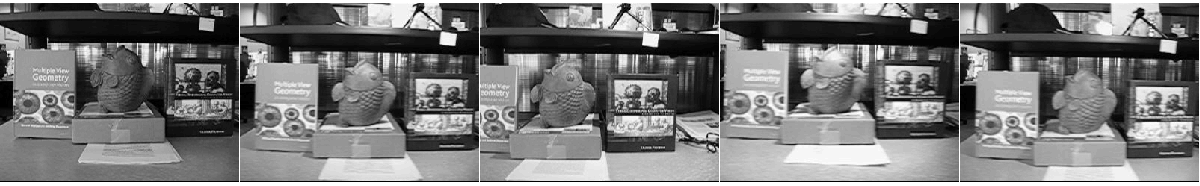
\includegraphics[height=0.41in]{thesis/seq_5_fish.png}\label{fig:trk_pca_1d}}
\subfigure{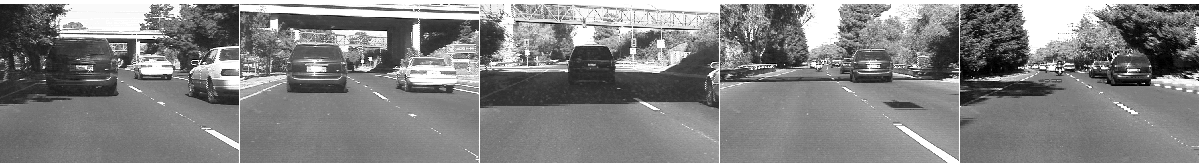
\includegraphics[height=0.41in]{thesis/seq_6_car4.png}\label{fig:trk_pca_1d}}
\subfigure{\includegraphics[height=0.41in]{thesis/seq_7_car11.png}\label{fig:trk_pca_1d}}
\label{fig:trk_sequences}
\end{figure}
\end{frame}

%------------------------------------------------------
\subsection{(a) Target representation}
%------------------------------------------------------
\begin{frame}
\frametitle{Target representation}
\framesubtitle{affine warping}
\logoCSIPCPL\mypagenum
\begin{equation*}
\begin{array}{cllll}
\left[\begin{array}{l}X\\Y\\1\end{array}\right]   &=& \AffMatrix \left[\begin{array}{l}x\\y\\1\end{array}\right]\\
\mathbf{\acute{x}} &=& \left[\begin{array}{cccc}\mathbf{A} & \mathbf{t}\\\mathbf{0}^T & 1\end{array}\right] \mathbf{x}\\
&=& \mathbf{A}\mathbf{x} + \mathbf{t}\\
&=& \mathbf{H}_A \mathbf{x}\\
\end{array}
\label{Eqn:top_level}
\end{equation*}
\end{frame}



\begin{frame}
\frametitle{Target representation}
\framesubtitle{inverse affine transform: one time initialization}
\logoCSIPCPL\mypagenum
In first frame
\begin{itemize}
\item given target affine parameters and ground truth feature points
\item apply inverse affine transform on ground truth points to warp them to canonical position, and save this position $(\mathbf{x, y})$
\end{itemize}
\begin{figure}[t]
\centering
\includegraphics[width=0.6\textwidth]{thesis/dataset_Dudek_00001_inverseAffine.pdf}
\label{fig:original_feature_points}
\end{figure}
\end{frame}




%------------------------------------------------------
\subsection{(b) Target motion}
%------------------------------------------------------
\begin{frame}
\frametitle{Target motion}
\framesubtitle{Generating track candidates: run-time}
\logoCSIPCPL\mypagenum
Use random affine deformation to model motion
\begin{itemize}
\item Perturb affine parameters
\item For each affine set, 
\begin{itemize}
\item apply forward affine transform on zero-centered canonical grid 
\item bilinear interpolation to extract ROI, one per affine set, as shown below
\begin{figure}[t]
\centering
\includegraphics[width=0.35\textwidth]{thesis/affineCandidates.pdf}
\label{Fig:affine_candidates}
\end{figure}
\end{itemize}
\item For set corresponding to least reconstruction error, apply forward affine transform to $(\mathbf{x, y})$ and compare with ground truth to get track error
\end{itemize}
\end{frame}








\begin{frame}[plain]
\frametitle{Target motion}
\framesubtitle{get ROI}
\logoCSIPCPL\mypagenum
\begin{changemargin}{-1.3in}{0in}
Density of grid points is greater in the horizontal direction.
\begin{figure}[t]
\centering
\fbox{\includegraphics[width=1.3\textwidth]{thesis/dataset_Dudek_00001_forwardAffine.pdf}}
\end{figure}
\end{changemargin}
\end{frame}


\begin{frame}
\frametitle{Target motion}
\framesubtitle{overlay feature points on ROI}
\logoCSIPCPL\mypagenum
\begin{itemize}
\item apply forward affine transform to canonical feature points $\mathbf{x,y}$ obtained in first frame
\item compare with ground truth
\item compute tracking error
\end{itemize}
\begin{figure}[t]
\centering
\includegraphics[width=0.55\textwidth]{thesis/dataset_Dudek_with_feature_points_00001.pdf}
\label{Fig:overall}
\end{figure}
\end{frame}

%------------------------------------------------------
\subsection{(c) Appearance model}
%------------------------------------------------------

%PCA
\begin{frame}
\frametitle{Appearance model}
\framesubtitle{PCA: 80/20 cross-validation, 10 runs, $\mathbb{R}^{1089}$}
\logoCSIPCPL\mypagenum
\setcounter{subfigure}{0}
\begin{figure}[t]
\subfigure[Uniform.]{\includegraphics[width=0.45\textwidth]{thesis/PCA_Uniform.pdf}}
\subfigure[Gaussian.]{\includegraphics[width=0.45\textwidth]{thesis/PCA_Gaussian.pdf}}
\subfigure[Gauss-Markov.]{\includegraphics[width=0.45\textwidth]{thesis/PCA_GaussMarkov.pdf}}
\subfigure[Dudek sequence.]{\includegraphics[width=0.45\textwidth]{thesis/PCA_Dudek.pdf}}
\label{fig:PCA_results}
\end{figure}
\end{frame}

%RVQ appearance model (varying P)
\begin{frame}
\frametitle{Appearance model}
\framesubtitle{RVQ, $M=4$, varying $P$: 80/20 cross-validation, 10 runs, $\mathbb{R}^{1089}$}
\mypagenum
\setcounter{subfigure}{0}
\begin{figure}
\subfigure[Uniform.]
{\includegraphics[width=0.45\textwidth]{thesis/RVQ_8x4_Uniform.pdf}}
\subfigure[Gaussian.]
{\includegraphics[width=0.45\textwidth]{thesis/RVQ_8x4_Gaussian.pdf}}
\subfigure[Gauss-Markov.]
{\includegraphics[width=0.45\textwidth]{thesis/RVQ_8x4_GaussMarkov.pdf}}
\subfigure[Dudek sequence.]
{\includegraphics[width=0.45\textwidth]{thesis/RVQ_8x4_Dudek.pdf}}
\end{figure}
\end{frame}


%TSVQ
\begin{frame}
\frametitle{Appearance model}
\framesubtitle{TSVQ (binary, balanced): 80/20 cross-validation, 10 runs, $\mathbb{R}^{1089}$}
\mypagenum
\setcounter{subfigure}{0}
\begin{figure}[t]
\subfigure[Uniform.]{\includegraphics[width=0.45\textwidth]{thesis/TSVQ_Uniform.pdf}}
\subfigure[Gaussian.]{\includegraphics[width=0.45\textwidth]{thesis/TSVQ_Gaussian.pdf}}
\subfigure[Gauss-Markov.]{\includegraphics[width=0.45\textwidth]{thesis/TSVQ_GaussMarkov.pdf}}
\subfigure[Dudek sequence.]{\includegraphics[width=0.45\textwidth]{thesis/TSVQ_Dudek.pdf}}
\label{fig:TSVQ_results}
\end{figure}
\end{frame}




%RVQ appearance model (varying M)
\begin{frame} 
\frametitle{Appearance model}
\framesubtitle{RVQ, $P=8$, varying $M$: 80/20 cross-validation, 10 runs, $\mathbb{R}^{1089}$}
\mypagenum
\setcounter{subfigure}{0}
\begin{figure}[t]
\subfigure[Uniform.]
{\includegraphics[width=0.45\textwidth]{thesis/RVQ_uniform.pdf}}
\subfigure[Gaussian.]
{\includegraphics[width=0.45\textwidth]{thesis/RVQ_Gaussian.pdf}}
\subfigure[Gauss-Markov.]
{\includegraphics[width=0.45\textwidth]{thesis/RVQ_GaussMarkov.pdf}}
\subfigure[Dudek sequence.]
{\includegraphics[width=0.45\textwidth]{thesis/RVQ_Dudek.pdf}}
\label{fig:RVQ_results_varyingM}
\end{figure}
\end{frame}



%------------------------------------------------------
\subsection{(d) Observation model}
%------------------------------------------------------
\begin{frame}
\frametitle{Observation model}
\framesubtitle{PCA}
\logoCSIPCPL\mypagenum
\begin{figure}
\centering
\includegraphics[width=0.75\textwidth]{thesis/PRML_PCA_problem.pdf}
\caption{In $\mathbb{R}^2$, a reduced eigenspace means that eigenvector $u_2$ is discarded.  Vectors $\mathbf{x}_1$ and $\mathbf{x}_2$ have the same projection error on eigenvector $u_1$ even though $\mathbf{x}_1$ is closer to the mean $\boldsymbol\mu$ of the training data $\mathbf{x}_i$.}
\label{fig:PRML_PCA_problem}
\end{figure}
\end{frame}


\begin{frame}
\frametitle{Observation model}
\framesubtitle{PCA}
\logoCSIPCPL\mypagenum
\begin{figure}[t]
\centering
\includegraphics[width=0.5\textwidth]{thesis/1998_JNL_ProbVisLearning_Moghaddam_fig3.png}
\caption{Graphical illustration of DFFS (distance-from-feature-space) and DIFS (distance-in-feature-space).  The feature space is $\mathbf{F}$ while the subspace orthogonal to the feature space is $\bar{\mathbf{F}}$.  DFFS is the signal residual error and DIFS is the $\mathbf{F}$-space likelihood \cite{1997_JNL_EigenTRK_Moghaddam}.}
\label{fig:1997_JNL_DIFSDFFS_Moghaddam}
\end{figure}
\end{frame}


\begin{frame}
\frametitle{Observation model}
\framesubtitle{PCA, RVQ, TSVQ}
\logoCSIPCPL\mypagenum
\begin{itemize}
\item PCA and RVQ both do not define a proper density in the observation space
\item For PCA, we use DFFS
\item For RVQ, we use
\begin{equation}
p(\mathbf{x}_i|\Phi) = \frac{e^{-\big(\dr\big)}} {\sum\limits_{i=1}^N e^{-\big(\dr\big)}}
\end{equation}
\item For TSVQ, the observation model is the same as RVQ with $\lambda=0$
\end{itemize}
\end{frame}


%------------------------------------------------------
\subsection{(e) State inference}
%------------------------------------------------------
\begin{frame}
\frametitle{State inference}
\framesubtitle{Particle filter: Sequential Importance Resampling Filter}
\mypagenum
\scriptsize
sampling is done in 6-D affine space

								\begin{figure}[t]
								\centering
								\subfigure[Reference (uniform) density and test PDF.]{\includegraphics[width=0.38\textwidth]{thesis/particle_filter_pdfs.pdf}}
								\subfigure[Comparing CDFs.]{\includegraphics[width=0.38\textwidth]{thesis/particle_filter_resampling.pdf}}
								\subfigure[Particles 4, 7 and 9 are picked repeatedly.]{\includegraphics[width=0.43\textwidth]{thesis/particle_filter_particles.pdf}}
								\caption{Particle filter, resampling.}
								\label{fig:particle_filter_resampling}
								\end{figure}
\end{frame}







%=======================================
\section{V. Results}
%=======================================

%-------------------------------------------------
\subsection{(a) Best performance}
%-------------------------------------------------
\begin{frame}
\frametitle{Results}
\framesubtitle{best tracking performance}
\logoCSIPCPL\mypagenum
\setcounter{subfigure}{0}
\begin{figure}[t]
\centering
\scriptsize
\begin{tabular}{|l|c|c|c|c|c|c|}
\hline
&\textbf{PCA}&\textbf{TSVQ}&\textbf{maxP}&\textbf{RofE}&\textbf{nulE}&\textbf{monR}\\\hline
\textbf{Dudek}&7.44&8.62&7.78&7.11&7.97&8.73\\\hline
\textbf{davidin300}&4.60&5.93&4.47&5.74&4.63&4.15\\\hline
\textbf{sylv}&4.34&4.61&4.00&4.12&4.74&4.31\\\hline
\textbf{fish}&2.17&4.59&2.78&2.73&2.48&2.89\\\hline
\textbf{car4}&4.60&5.11&4.67&4.93&5.28&4.71\\\hline
\textbf{car11}&2.13&2.21&2.17&2.33&2.52&2.47\\\hline
\textbf{ \% best}&50.00&0.00&16.67&16.67&0.00&16.67\\\hline
\end{tabular}

\subfigure[Best tracking error for each algorithm.]{\includegraphics[width=0.47\textwidth]{thesis/results_final_1a_best.pdf}\label{fig:results_final_1a_best}}\hspace{0.1in}
\subfigure[\%age of datasets over which best tracking error is achieved over all parameters.]{\includegraphics[width=0.47\textwidth]{thesis/results_final_1b_best_percent.pdf}\label{fig:results_final_1b_best_percent}}
\end{figure}
\end{frame}

%-------------------------------------------------
\subsection{(b) Mean performance over params.}
%-------------------------------------------------

\begin{frame}
\frametitle{Results}
\framesubtitle{mean performance}
\logoCSIPCPL\mypagenum
\setcounter{subfigure}{0}
\begin{figure}[t]
\centering
\scriptsize
\begin{tabular}{|l|c|c|c|c|c|c|}
\hline
&\textbf{PCA}&\textbf{TSVQ}&\textbf{maxP}&\textbf{RofE}&\textbf{nulE}&\textbf{monR}\\\hline
\textbf{Dudek}&7.93&10.07&7.93&7.91&8.60&9.90\\\hline
\textbf{davidin300}&6.63&8.37&7.07&6.99&5.72&4.99\\\hline
\textbf{sylv}&5.18&4.70&4.47&4.83&5.10&4.66\\\hline
\textbf{fish}&6.63&6.71&8.81&5.97&5.74&6.15\\\hline
\textbf{car4}&4.97&5.90&5.38&5.19&5.77&4.99\\\hline
\textbf{car11}&2.24&3.48&2.70&2.49&2.69&2.58\\\hline
\textbf{ \% best}&33.33&0.00&16.67&16.67&16.67&16.67\\\hline
\end{tabular}

\subfigure[Mean tracking error for each algorithm.]{\includegraphics[width=0.47\textwidth]{thesis/results_final_2a_mean.pdf}\label{fig:results_final_2a_mean}}\hspace{0.1in}
\subfigure[\%age of datasets over which best mean tracking error is achieved over all parameters.]{\includegraphics[width=0.47\textwidth]{thesis/results_final_2b_mean_percent.pdf}\label{fig:results_final_2b_mean_percent}}
\label{fig:results_final_2_mean}
\end{figure}
\end{frame}

%-------------------------------------------------
\subsection{(c) Memory=16 vectors}
%-------------------------------------------------

\begin{frame}
\frametitle{Results}
\framesubtitle{memory=16 vectors}
\logoCSIPCPL\mypagenum
\setcounter{subfigure}{0}
\begin{figure}[t]
\centering
\scriptsize
\begin{tabular}{|l|c|c|c|c|c|c|}
\hline
&\textbf{PCA}&\textbf{TSVQ}&\textbf{maxP}&\textbf{RofE}&\textbf{nulE}&\textbf{monR}\\\hline
\textbf{Dudek}&7.81&8.62&7.78&7.11&9.65&11.81\\\hline
\textbf{davidin300}&4.60&12.88&6.84&9.02&7.17&50.00\\\hline
\textbf{sylv}&5.47&4.70&4.00&4.12&4.81&4.31\\\hline
\textbf{fish}&2.17&10.07&11.50&2.96&4.03&2.89\\\hline
\textbf{car4}&4.60&5.11&4.67&4.93&5.28&5.07\\\hline
\textbf{car11}&2.13&2.21&2.17&2.47&2.59&2.47\\\hline
\textbf{ \% best}&66.67&0.00&16.67&16.67&0.00&0.00\\\hline
\end{tabular}

\subfigure[Tracking error for each algorithm with 16 eigenvectors/code-vectors stored in memory.]{\includegraphics[width=0.47\textwidth]{thesis/results_final_3a_16.pdf}\label{fig:results_final_3a_16}}\hspace{0.1in}
\subfigure[\%age of datasets over which best tracking error is achieved with 16 eigenvectors/code-vectors stored in memory.]{\includegraphics[width=0.47\textwidth]{thesis/results_final_3b_16_percent.pdf}\label{fig:results_final_3b_16_percent}}
\label{fig:results_final_3_16}
\end{figure}
\end{frame}


%-------------------------------------------------
\subsection{(d) Memory=32 vectors}
%-------------------------------------------------
\begin{frame}
\frametitle{Results}
\framesubtitle{memory=32 vectors}
\logoCSIPCPL\mypagenum
\setcounter{subfigure}{0}
\begin{figure}[t]
\centering
\scriptsize
\begin{tabular}{|l|c|c|c|c|c|c|}
\hline
&\textbf{PCA}&\textbf{TSVQ}&\textbf{maxP}&\textbf{RofE}&\textbf{nulE}&\textbf{monR}\\\hline
\textbf{Dudek}&8.54&11.87&7.92&8.43&8.19&9.17\\\hline
\textbf{davidin300}&6.93&6.29&4.47&6.21&5.35&5.83\\\hline
\textbf{sylv}&5.72&4.80&4.68&5.54&5.74&4.58\\\hline
\textbf{fish}&7.98&4.59&2.78&12.22&2.48&3.62\\\hline
\textbf{car4}&5.52&6.79&6.38&5.14&5.84&5.18\\\hline
\textbf{car11}&2.39&5.28&2.36&2.33&2.52&2.72\\\hline
\textbf{ \% best}&0.00&0.00&33.33&33.33&16.67&16.67\\\hline
\end{tabular}

\subfigure[Tracking error for each algorithm with 32 eigenvectors/code-vectors stored in memory.]{\includegraphics[width=0.47\textwidth]{thesis/results_final_4a_32.pdf}\label{fig:results_final_4a_32}}\hspace{0.1in}
\subfigure[\%age of datasets over which best tracking error is achieved with 32 eigenvectors/code-vectors stored in memory.]{\includegraphics[width=0.47\textwidth]{thesis/results_final_4b_32_percent.pdf}\label{fig:results_final_4b_32_percent}}
\label{fig:results_final_4_32}
\end{figure}
\end{frame}


%-------------------------------------------------
\subsection{(e) Mean performance over datasets}
%-------------------------------------------------
\begin{frame}
\frametitle{Results}
\framesubtitle{over all configurations}
\logoCSIPCPL\mypagenum
\setcounter{subfigure}{0}
\vspace{-0.2in}
\begin{figure}[h!]
\centering
\subfigure[PCA.]{\includegraphics[width=0.225\textwidth, angle=90]{thesis/results_final_5a_pca_.pdf}\label{fig:results_final_5a_pca_}}
\subfigure[TSVQ.]{\includegraphics[width=0.225\textwidth, angle=90]{thesis/results_final_5b_tsvq.pdf}\label{fig:results_final_5b}}
\subfigure[maxP.]{\includegraphics[width=0.3\textwidth]{thesis/results_final_5c_maxP.pdf}\label{fig:results_final_5c}}
\subfigure[RofE.]{\includegraphics[width=0.3\textwidth]{thesis/results_final_5d_RofE.pdf}\label{fig:results_final_5d}}
\subfigure[nulE.]{\includegraphics[width=0.3\textwidth]{thesis/results_final_5e_nulE.pdf}\label{fig:results_final_5e}}
\subfigure[monR.]{\includegraphics[width=0.3\textwidth]{thesis/results_final_5f_monR.pdf}\label{fig:results_final_5f}}
\subfigure[maxP, RofE, nulE, monR.]{\includegraphics[width=0.3\textwidth]{thesis/results_final_5g_8x2_8x4_8x8.pdf}\label{fig:results_final_5g_8x2_8x4_8x8}}
\caption{Tracking results (5 of 5), comparison of tracking performance as parameters for each algorithm are varied.  In (d), we see that over all RVQ algorithms, RofE has best mean performance.  In (g) it is clear that the best RVQ configuration is 8x4.}
\label{fig:results_final_5_configs}
\end{figure}
\end{frame}

%=======================================
\section{VI. Conclusions}
%=======================================
\begin{frame}
\frametitle{Conclusions}
\framesubtitle{}
\logoCSIPCPL\mypagenum
\begin{itemize}
\item \underline{Best possible performance}.  PCA and RVQ performed best in half the times each.  TSVQ never performed best.  However, of the 3 times that PCA performed best, in 2 cases, the performance difference was not significantly better than RVQ.  Moreover, and perhaps more importantly, RVQ performed best in the two most challenging datasets, Dudek and davidin300 since they both have multiple sources of noise.
\item \underline{Best mean performance}.  Here, RVQ performed best in twice the number of scenarios as PCA.  TSVQ had the worst mean performance.
\end{itemize}
\end{frame}

\begin{frame}
\frametitle{Conclusions}
\framesubtitle{}
\logoCSIPCPL\mypagenum
\begin{itemize}
\item \underline{Memory cost=16 vectors}.  Here PCA performed best in twice the number of scenarios as RVQ .
\item \underline{Memory cost=32 vectors}.  Here RVQ completely outperformed PCA and TSVQ.  This is understandable since the capacity of RVQ to explain an underlying distribution grows exponentially as $M^P$.  Moreover, we have used $M=2, 4, 8$ ensuring that we do not increase our VC dimension too much so as to start over-fitting
\item \underline{Lost tracks}.  There was only one lost track for monR.  This is understandable since monR is a greedy approach.  The lost track was in davidin300 which is a challenging dataset.
\end{itemize}
\end{frame}

\begin{frame}
\frametitle{Conclusions}
\framesubtitle{}
\logoCSIPCPL\mypagenum
\begin{itemize}
\item If dataset has different forms of noise, such as blur, lighting change, pose change, then RVQ performs better
\item If dataset has one form of noise, such as lighting change, then PCA performs better
\item Reason is that for PCA, first eigenvector explains maximum variance
\item Subsequent eigenvectors are constrained
\item RVQ is not constrained
\end{itemize}
\end{frame}


\begin{frame}
\frametitle{Future work}
\framesubtitle{}
\logoCSIPCPL\mypagenum
\setcounter{subfigure}{0}
\begin{enumerate}
\item Compare with non-linear manifold learning methods
\item Relationship to Ding and He, 2004
\item Multi-spectral data
\item Multi-target
\item Increase stage refinement in RVQ
\end{enumerate}
\end{frame}

%=======================================
\section{Questions}
%=======================================
\begin{frame}
\frametitle{Open source}
\framesubtitle{}
\logoCSIPCPL\mypagenum
\setcounter{subfigure}{0}
\begin{itemize}
\item All PhD work released under open source license
\item git clone, or download as zip
{\color{blue}\underline{\url{https://github.com/SalmanAslamPhD/phd}}}
\begin{figure}
\includegraphics[width=0.9\textwidth]{thesis/github.png}
\end{figure}
\item To run tracker, run main.m
\end{itemize}
\end{frame}

\begin{frame}
\frametitle{}
\logoCSIPCPL\mypagenum
		QUESTIONS
\begin{figure}
\includegraphics[width=1.0\textwidth]{thesis/00465.png}
\end{figure}

\end{frame}

%####################################################################################################
%####################################################################################################
%\bibliographystyle{ieee}
%\bibliography{c:/salman/work/writing/MyCitations}
\end{document}
%####################################################################################################

%####################################################################################################

